
\chapter{核力\label{chap:=006838=00529B}}

\section{引言}

到目前为止，我们只定性地考虑了核子间的作用力。我们用它们的某些性质——如短程性和饱和性——来解释液滴模型中的体积项和表面项。我们还假定它们给出了一个平均单粒子势。通过调整一些参数，我们能够复现大量的实验数据，这些唯象模型的成功使我们有信心进一步从更微观的角度研究核多体问题。另外，我们也希望应用现代多体理论的技术。

所有这些考虑的出发点显然是核子之间的两体相互作用。在这个概念中有三个基本假设：
\begin{enumerate}
\item 介子的动力学自由度可以忽略不计，原子核可以描述为$A$核子系统，其相互作用可以用势表示。
\item 相对论效应可以忽略不计。
\item 只有两体力是重要的。
\end{enumerate}
即使有了这些相当极端的假设，当我们试图按照我们讨论过的方式继续下去时，我们也会立即遇到两个困难：

第一，不存在从第一性原理导出核力的方法。虽然这在夸克和胶子规范场的现代理论中原则上是可能的，但在这方面的尝试还只是在起步阶段\cite{De78}。另一方面，从相互作用介子和核子的有效拉格朗日量出发的理论最近被证明是相当成功的（参见，例如，{[}CLL
73，LLR 75，DSB 77，Vi 78，Ho 80{]}）。这种核力的基本成分是$\pi$-核子耦合常数，这是从实验中得知的。当核子间距大于$0.8\,\text{fm}$时，这种核力没有自由参数，而从$0$到$0.8\,\text{fm}$的部分则由一个每个同位旋自由度上包含六个参数的唯象势表示，它最终很好地拟合了所测得的核子-核子相移。

迄今为止使用的核力几乎完全是唯象的（除了由单$\pi$介子交换产生的 Yukawa 势外；见下文），并包含多达约$50$个参数。这些核力很好的复现了实验上测得的相移。在这些核力的基础上，我们将在第4.2.2节非常简要地讨论如何应用多体理论的方法以定量的方式导出前面几章讨论的唯象性质。

然而，原子核理论中还有第二个困难。那就是从数值的观点来看，这些裸核力的行为非常病态。它们在短程内表现出很强的排斥行为（排斥芯）从而不能直接用一些多体方法来处理。例如，对于微扰论来说，这相互作用太强了，而对于自洽场方法（第五章）来说，排斥芯几乎是不可能处理的。事实上，核内的核子感受不到裸的核力，因为它们是在许多其他核子存在的情况下相互作用的，这允许我们引入所谓的有效核子-核子相互作用。这种相互作用表现得相当好，并允许我们应用通常的多体方法，如Hartree-Fock理论（第5章）。人们已经做了大量的工作，从裸核子-核子相互作用力导出这种有效相互作用。在4.3节我们讨论了为实现这一目标所采用的基本思想。迄今为止，人们对这些有效核力的性质和结构已经有了大量的了解。然而，为了定量地再现实验数据，人们仍然需要唯象的调整这些参数，从这个角度来看，这一理论还不是很令人满意。

在大多数所谓的原子核微观描述中，人们使用唯象的有效核力，这些有效核力是基于这些考虑而构建的，但仍然有一些可调节的用来适应实验数据的参数。

在这一章我们并不想尝试去推导裸核力\cite{BJ76a}。在第二节我们将会讨论裸核力有的一些对称性，这使得我们可以推导一些结论。第三节我们简要介绍了有效相互作用的微观描述，讨论了它们的性质和应用领域。第四节介绍了一些用于描述一个给定平均势中运动核子间的剩余相互作用的唯象势。

需要强调的是，在这一章中我们只讨论核力，而库仑力必须单独讨论。当需要与实验数据进行比较时，必须首先减去库仑效应。

\section{裸核力\label{sec:=0088F8=006838=00529B}}

\subsection{两体力的一般性质}

量子力学中最一般的两体相互作用$V$可以由其夹在两粒子态（坐标表象下是$|\boldsymbol{r}_{1},s_{1},t_{1};\boldsymbol{r}_{2},s_{2},t_{2}\rangle$，这里$s_{i}=\pm\frac{1}{2}$是自旋，$t_{i}=\pm\frac{1}{2}$是同位旋）间得到的矩阵元完全确定：
\[
\langle\boldsymbol{r}^{\prime}_{1}s^{\prime}_{1}t^{\prime}_{1}\boldsymbol{r}^{\prime}_{2}s^{\prime}_{2}t^{\prime}_{2}|V|\boldsymbol{r}_{1}s_{1}t_{1}\boldsymbol{r}_{2}s_{2}t_{2}\rangle
\]

两粒子态$|\boldsymbol{r}_{1},s_{1},t_{1};\boldsymbol{r}_{2},s_{2},t_{2}\rangle$的空间是空间波函数$|\boldsymbol{r}_{1}\rangle$和$|\boldsymbol{r}_{2}\rangle$，自旋和同位旋态矢$|s_{1}\rangle,|s_{2}\rangle$和$|t_{1},t_{2}\rangle$的直积。由于自旋空间的任意算符都可以表示为Pauli矩阵$\sigma_{1}$，$\sigma_{2}$，$\sigma_{3}$和单位矩阵$\sigma_{0}$的线性组合
\begin{comment}
这一结论依赖于厄米性，而本书中后面又把厄米性当做单独的对称性，是一种逻辑混乱。
\end{comment}
，因此最一般的形式是：
\begin{equation}
V=\sum^{3}_{i,j=0}V_{ij}\sigma^{(1)}_{i}\sigma^{(2)}_{j}\label{eq:general V in spin space}
\end{equation}

类似地，$V_{ij}$也这么依赖于同位旋算符$\boldsymbol{\tau}^{(1)}$和$\boldsymbol{\tau}^{(2)}$。除了这一同位旋依赖性，坐标空间的$V_{ij}$是积分算符：
\begin{equation}
V|\boldsymbol{r}_{1}\boldsymbol{r}_{2}\rangle=\int V(\boldsymbol{r}^{\prime}_{1},\boldsymbol{r}^{\prime}_{2},\boldsymbol{r}_{1},\boldsymbol{r}_{2})|\boldsymbol{r}^{\prime}_{1}\boldsymbol{r}^{\prime}_{2}\rangle\,\mathrm{d}^{3}\boldsymbol{r}^{\prime}_{1}\mathrm{d}^{3}\boldsymbol{r}^{\prime}_{2}\label{eq:V in coordinate space}
\end{equation}

特殊情况下，$V(\boldsymbol{r}^{\prime}_{1},\boldsymbol{r}^{\prime}_{2},\boldsymbol{r}_{1},\boldsymbol{r}_{2})$具有如下形式：
\[
V(\boldsymbol{r}_{1},\boldsymbol{r}_{2},\boldsymbol{r}^{\prime}_{1},\boldsymbol{r}^{\prime}_{2})=\delta(\boldsymbol{r}_{1}-\boldsymbol{r}^{\prime}_{1})\delta(\boldsymbol{r}_{2}-\boldsymbol{r}^{\prime}_{2})V(\boldsymbol{r}_{1},\boldsymbol{r}_{2})
\]

这时$V$被称为局域势，我们有：
\[
V|\boldsymbol{r}_{1}\boldsymbol{r}_{2}\rangle=V(\boldsymbol{r}_{1},\boldsymbol{r}_{2})|\boldsymbol{r}_{1}\boldsymbol{r}_{2}\rangle
\]

在这种情况下，两粒子相互作用仅仅依赖于$\boldsymbol{r}_{1}$和$\boldsymbol{r}_{2}$（当然也依赖于自旋和同位旋）。它并不依赖于如粒子的速度这样的量。

我们需要说明，一般来讲，非局域的势是速度依赖的。我们把$|\boldsymbol{r}^{\prime}_{1}\boldsymbol{r}^{\prime}_{2}\rangle$展开\footnote{这里$:\mathrel{}:$是正规序，意思是说$\partial/\partial\boldsymbol{r}_{i}$不作用到指数展开项的$\boldsymbol{r}_{i}$上。}：

\begin{align*}
|\boldsymbol{r}^{\prime}_{1},\boldsymbol{r}^{\prime}_{2}\rangle & =|\boldsymbol{r}_{1}\boldsymbol{r}_{2}\rangle+(\boldsymbol{r}^{\prime}_{1}-\boldsymbol{r}_{1})\frac{\partial}{\partial\boldsymbol{r}_{1}}|\boldsymbol{r}_{1}\boldsymbol{r}_{2}\rangle+(\boldsymbol{r}^{\prime}_{2}-\boldsymbol{r}_{2})\frac{\partial}{\partial\boldsymbol{r}_{2}}|\boldsymbol{r}_{1}\boldsymbol{r}_{2}\rangle+\dots\\
 & =:\mathrel{\exp\left((\boldsymbol{r}^{\prime}_{1}-\boldsymbol{r}_{1})\frac{\partial}{\partial\boldsymbol{r}_{1}}+(\boldsymbol{r}^{\prime}_{2}-\boldsymbol{r}_{2})\frac{\partial}{\partial\boldsymbol{r}_{2}}\right)}:|\boldsymbol{r}_{1}\boldsymbol{r}_{2}\rangle
\end{align*}

由\ref{eq:V in coordinate space}可以得到：
\begin{align*}
V|\boldsymbol{r}_{1}\boldsymbol{r}_{2}\rangle & =\int V(\boldsymbol{r}^{\prime}_{1},\boldsymbol{r}^{\prime}_{2},\boldsymbol{r}_{1},\boldsymbol{r}_{2})\exp\left(\frac{\mathrm{i}}{\hbar}(\boldsymbol{r}^{\prime}_{1}-\boldsymbol{r}_{1})\boldsymbol{p}_{1}+\frac{\mathrm{i}}{\hbar}(\boldsymbol{r}^{\prime}_{2}-\boldsymbol{r}_{2})\boldsymbol{p}_{2}\right)|\boldsymbol{r}_{1}\boldsymbol{r}_{2}\rangle\,\mathrm{d}^{3}\boldsymbol{r}^{\prime}_{1}\mathrm{d}^{3}\boldsymbol{r}^{\prime}_{2}\\
 & =\tilde{V}(\boldsymbol{r}_{1},\boldsymbol{p}_{1},\boldsymbol{r}_{2},\boldsymbol{p}_{2})|\boldsymbol{r}_{1}\boldsymbol{r}_{2}\rangle
\end{align*}

这意味着最一般的势可以用\ref{eq:general V in spin space}表示，里面的$V_{ij}$在坐标空间中具有上式的形式（为了简化我们忽略了同位旋依赖性）。

接下来我们讨论核力$V(1,2)=V(\boldsymbol{r}_{1},\boldsymbol{p}_{1},\boldsymbol{\sigma}^{(1)},\boldsymbol{\tau}^{(1)},\boldsymbol{r}_{2},\boldsymbol{p}_{2},\boldsymbol{\sigma}^{(2)},\boldsymbol{\tau}^{(2)})$的对称性。通过给定一系列的对称性，这一普适的函数形式会被限制。

这里我们给定了八种对称性：
\begin{enumerate}
\item 厄米性
\item 置换对称性
\[
V(1,2)=V(2,1)
\]

这一性质和两粒子波函数的对称性相关。由于核子是费米子，它们具有反对称性。例如，如果我们写出一个坐标空间，自旋空间和同位旋空间的直积波函数：
\[
\langle\boldsymbol{r}_{1}s_{1}t_{1},\boldsymbol{r}_{2}s_{2}t_{2}|12\rangle=\varphi(\boldsymbol{r}_{1},\boldsymbol{r}_{2})\chi(s_{1},s_{2})\zeta(t_{1},t_{2})
\]

我们有四种符合泡利原理的组合，它们可以通过坐标空间和自旋部分的对称性来标记\ref{tab:=004E24=007C92=005B50=006001=005BF9=0079F0=006027=007684=005206=007C7B}，在每种情况下，同位旋分量都是通过总波函数的反对称性来确定的。
\begin{table}[H]
\begin{centering}
\caption{\label{tab:=004E24=007C92=005B50=006001=005BF9=0079F0=006027=007684=005206=007C7B}两粒子态对称性的分类}
\par\end{centering}
\centering{}%
\begin{tabular}{|c|c|c|c|}
\hline 
$\varphi$ & $\chi$ & 缩写 & $\zeta$\tabularnewline
\hline 
\hline 
偶 & 单态 & es & $+$\tabularnewline
\hline 
偶 & 三重态 & et & $-$\tabularnewline
\hline 
奇 & 单态 & os & $-$\tabularnewline
\hline 
奇 & 三重态 & ot & $+$\tabularnewline
\hline 
\end{tabular}
\end{table}

\item 平移不变性。核力只依赖于相对坐标：
\[
V(1,2)=V(\boldsymbol{r},\boldsymbol{p}_{1},\boldsymbol{\sigma}^{(1)},\boldsymbol{\tau}^{(1)},\boldsymbol{p}_{2},\boldsymbol{\sigma}^{(2)},\boldsymbol{\tau}^{(2)})
\]
\item 伽利略不变性。核力在惯性参考系之间的变换下不变，即只依赖于相对动量$\boldsymbol{p}=\frac{1}{2}(\boldsymbol{p}_{1}-\boldsymbol{p}_{2})$：
\[
V(1,2)=V(\boldsymbol{r},\boldsymbol{p},\boldsymbol{\sigma}^{(1)},\boldsymbol{\tau}^{(1)},\boldsymbol{\sigma}^{(2)},\boldsymbol{\tau}^{(2)})
\]
\item 空间反演不变性。和弱相互作用不同，强相互作用是宇称守恒的：
\[
V(\boldsymbol{r},\boldsymbol{p},\boldsymbol{\sigma}^{(1)},\boldsymbol{\tau}^{(1)},\boldsymbol{\sigma}^{(2)},\boldsymbol{\tau}^{(2)})=V(-\boldsymbol{r},-\boldsymbol{p},\boldsymbol{\sigma}^{(1)},\boldsymbol{\tau}^{(1)},\boldsymbol{\sigma}^{(2)},\boldsymbol{\tau}^{(2)})
\]
\item 时间反演不变性。它保证了运动方程不依赖于时间演化的方向（细节参考\cite{Me61}）。
\[
V(\boldsymbol{r},\boldsymbol{p},\boldsymbol{\sigma}^{(1)},\boldsymbol{\tau}^{(1)},\boldsymbol{\sigma}^{(2)},\boldsymbol{\tau}^{(2)})=V(\boldsymbol{r},-\boldsymbol{p},-\boldsymbol{\sigma}^{(1)},\boldsymbol{\tau}^{(1)},-\boldsymbol{\sigma}^{(2)},\boldsymbol{\tau}^{(2)})
\]
\item 空间转动不变性。三维空间转动不仅仅作用在$\boldsymbol{r}$和$\boldsymbol{p}$上，也作用在自旋矩阵$\boldsymbol{\sigma}=2\cdot\boldsymbol{s}$上。算符$V$在自旋空间必须具有\ref{eq:general V in spin space}的形式。它必须在空间转动下是标量，这意味着$V_{00}$必须是个标量。我们从$\boldsymbol{r}$和$\boldsymbol{p}$可以构建三个独立的标量$r^{2}$，$p^{2}$和$\boldsymbol{r}\cdot\boldsymbol{p}+\boldsymbol{p}\cdot\boldsymbol{r}$。由于时间反演不变性，后一个表达式只能以二次的形式出现。因此一种更方便的方法是把$(\boldsymbol{r}\cdot\boldsymbol{p}+\boldsymbol{p}\cdot\boldsymbol{r})^{2}$用$r^{2}$，$p^{2}$和$L^{2}=(\boldsymbol{r}\times\boldsymbol{p})^{2}$表示出来。$V_{00}$可以写成$r^{2}$，$p^{2}$和$L^{2}$的函数。由于置换对称性和空间反演不变性我们发现：
\[
V(\boldsymbol{r},\boldsymbol{p},\boldsymbol{\sigma}^{(1)},\boldsymbol{\sigma}^{(2)})=V(\boldsymbol{r},\boldsymbol{p},\boldsymbol{\sigma}^{(2)},\boldsymbol{\sigma}^{(1)})
\]

因此\ref{eq:general V in spin space}中的线性项只依赖于：
\[
\boldsymbol{S}=\frac{1}{2}(\boldsymbol{\sigma}^{(1)}+\boldsymbol{\sigma}^{(2)})
\]

为了形成一个标量，$\boldsymbol{S}$必须和一个矢量相乘，此外还要考虑空间反演不变性，只有$\boldsymbol{L}$满足这一要求：
\[
\boldsymbol{L}\cdot\boldsymbol{S}=\frac{1}{2}\boldsymbol{L}\cdot(\boldsymbol{\sigma}^{(1)}+\boldsymbol{\sigma}^{(2)})
\]

\ref{eq:general V in spin space}中的二次项形成了一个张量，。它可以分解成一个标量$\boldsymbol{\sigma}^{(1)}\cdot\boldsymbol{\sigma}^{(2)}$，一个矢量$\boldsymbol{\sigma}^{(1)}\times\boldsymbol{\sigma}^{(2)}$，一个无迹对称张量$(\sigma^{(1)}_{i}\sigma^{(2)}_{k}+\sigma^{(1)}_{k}\sigma^{(2)}_{i})(1-\frac{1}{3}\delta_{ik})$。根据Okubo和Marshak\cite{OM58}的研究，$\boldsymbol{\sigma}^{(1)}\times\boldsymbol{\sigma}^{(2)}$不能出现，所有可能的组合是：
\[
\boldsymbol{\sigma}^{(1)}\cdot\boldsymbol{\sigma}^{(2)},(\boldsymbol{r}\cdot\boldsymbol{\sigma}^{(1)})(\boldsymbol{r}\cdot\boldsymbol{\sigma}^{(2)}),(\boldsymbol{p}\cdot\boldsymbol{\sigma}^{(1)})(\boldsymbol{p}\cdot\boldsymbol{\sigma}^{(2)}),(\boldsymbol{L}\cdot\boldsymbol{\sigma}^{(2)})(\boldsymbol{L}\cdot\boldsymbol{\sigma}^{(2)})+(\boldsymbol{L}\cdot\boldsymbol{\sigma}^{(2)})(\boldsymbol{L}\cdot\boldsymbol{\sigma}^{(1)})
\]

所有这些项都可以与$r^{2}$，$p^{2}$和$L^{2}$的任意函数相乘。
\item 同位旋空间的转动不变性。在同位旋的框架下，质子和中子被视为一种可以形成同位旋$\frac{1}{2}$双重态的基本粒子。转动群的二维表示即可刻画它们所有的变换性质。同位旋空间的转动（只要它们不是沿着第三个轴
\begin{comment}
这句话是什么意思？
\end{comment}
）产生了质子中子的混合态。核力的转动不变性因此意味着电荷无关性，也就是质子质子相互作用和中子中子相互作用相同。这可以从核子核子散射实验和镜像核（例如$\text{He}^{3}$和$\text{H}^{3}$）的性质得出。数学上讲，这意味着核力$V(1,2)$和总同位旋算符$\boldsymbol{T}=\boldsymbol{t}_{1}+\boldsymbol{t}_{2}$交换。因此本征态可以通过$T^{2}$，$T_{3}$对应的本征值为$T=0$，$T_{3}=0$和$T=1$，$T_{3}=-1,0,+1$的态（同位旋单重态和三重态）构造出来。电荷无关性意味着$T^{2}$与核力算符对易。因此，$T=1$态的相互作用（pp，nn或者对称的pn态）必须是一样的。然而，$T=0$的态可能是不同的。

同位旋矩阵$\boldsymbol{\tau}=(\tau_{1},\tau_{2},\tau_{3})$的形式和通常的自旋矩阵相同。由于同位旋空间没有其它矢量，因此仅有的同位旋转动不变的粒子1和2的组合是：
\[
V_{0}+V_{\tau}\boldsymbol{\tau}^{(1)}\cdot\boldsymbol{\tau}^{(2)}
\]

正如我们已经讨论的$V_{0}$和$V_{\tau}$依赖于剩余的坐标例如$\boldsymbol{r}$，$\boldsymbol{p}$，$\boldsymbol{\sigma}_{1}$，$\boldsymbol{\sigma}_{2}$。
\end{enumerate}
不是所有对称性允许的组合都被用来描述核力，我们这里只涉及一些重要的项：
\begin{enumerate}
\item 局域的，即不依赖于速度的势中，中心力是最重要的。它仅仅依赖于核子间的距离$r$：
\begin{equation}
V_{\text{C}}(1,2)=V_{0}(r)+V_{\sigma}(r)\boldsymbol{\sigma}^{(1)}\cdot\boldsymbol{\sigma}^{(2)}+V_{\tau}(r)\boldsymbol{\tau}^{(1)}\cdot\boldsymbol{\tau}^{(2)}+V_{\sigma\tau}(r)(\boldsymbol{\sigma}^{(1)}\cdot\boldsymbol{\sigma}^{(2)})(\boldsymbol{\tau}^{(1)}\cdot\boldsymbol{\tau}^{(2)})\label{eq:center force}
\end{equation}
\item 剩余的局域势是张量力：
\[
V_{T}(1,2)=[V_{T_{0}}(r)+V_{T}(r)\boldsymbol{\tau}^{(1)}\cdot\boldsymbol{\tau}^{(2)}]\boldsymbol{S}_{12}
\]

这里：
\[
S_{12}=\frac{3}{r^{2}}(\boldsymbol{\sigma}^{(1)}\cdot\boldsymbol{r})(\boldsymbol{\sigma}^{(2)}\cdot\boldsymbol{r})-\boldsymbol{\sigma}^{(1)}\cdot\boldsymbol{\sigma}^{(2)}
\]

$-\boldsymbol{\sigma}^{(1)}\cdot\boldsymbol{\sigma}^{(2)}$这一项添加是为了保证$V_{T}(1,2)$对所有的方向积分为零：
\[
\int V_{T}(1,2)\,\mathrm{d}\Omega=0\quad\text{这里}\boldsymbol{r}=(r,\Omega)
\]

实验上关于核子核子间张量力存在的证据是氚核的四极矩，这是不能被单纯的中心力解释的。
\item 最重要的非局域势是两体自旋轨道相互作用：
\[
V_{LS}=V_{LS}(r)\boldsymbol{L}\cdot\boldsymbol{S}
\]

正如我们在第五章将会看到的，这样的一个两体自旋轨道耦合项导致了平均单粒子势中的单体自旋轨道耦合项，可以被用来解释原子核中的幻数。
\item 有时候我们也用二阶的自旋轨道相互作用：
\[
V_{LL}=V_{LL}(r)\left\{ (\boldsymbol{\sigma}^{(1)}\cdot\boldsymbol{\sigma}^{(2)})L^{2}-\frac{1}{2}\left[(\boldsymbol{\sigma}^{(1)}\cdot\boldsymbol{L})(\boldsymbol{\sigma}^{(2)}\cdot\boldsymbol{L})+(\boldsymbol{\sigma}^{(2)}\cdot\boldsymbol{L})(\boldsymbol{\sigma}^{(1)}\cdot\boldsymbol{L})\right]\right\} 
\]
\end{enumerate}

\subsection{核力的结构}

中心力是核子核子相互作用中最重要的部分。它也可以用一些交换或者投影算符来表示。

下面的算符可以交换波函数中的自旋和同位旋坐标：
\begin{align*}
P^{\sigma} & =\frac{1}{2}(1+\boldsymbol{\sigma}^{(1)}\cdot\boldsymbol{\sigma}^{(2)})\\
P^{\tau} & =\frac{1}{2}(1+\boldsymbol{\tau}^{(1)}\cdot\boldsymbol{\tau}^{(2)})
\end{align*}

我们把$P^{\sigma}$作用到波函数上即可得到：

\[
P^{\sigma}\varphi(\boldsymbol{r}_{1},\boldsymbol{r}_{2})\chi(s_{1},s_{2})\zeta(t_{1},t_{2})=\varphi(\boldsymbol{r}_{1},\boldsymbol{r}_{2})\chi(s_{2},s_{1})\zeta(t_{1},t_{2})
\]

这可以很容易的通过总自旋算符$\boldsymbol{S}$算符理解。$S^{2}$算符的本征态是单态或者三重态：

\[
P^{\sigma}=\frac{1}{2}[1+2(S^{2}-s^{(1)2}-s^{(2)2})]=S(S+1)-1=\begin{cases}
1 & \text{三重态}\\
-1 & \text{单态 }
\end{cases}
\]

我们也可以定义一个算符$P^{r}$交换粒子的空间坐标$\boldsymbol{r}_{1}$和$\boldsymbol{r}_{2}$。

\footnote{这一算符可以在坐标空间用一个非局域的算符表示：
\[
V(\boldsymbol{r})P^{r}\psi(\boldsymbol{r}_{1},\boldsymbol{r}_{2})=\int V(\boldsymbol{r}_{1}-\boldsymbol{r}_{2})\delta(\boldsymbol{r}^{\prime}_{1}-\boldsymbol{r}_{2})\delta(\boldsymbol{r}^{\prime}_{2}-\boldsymbol{r}_{1})\psi(\boldsymbol{r}^{\prime}_{1},\boldsymbol{r}^{\prime}_{2})\,\mathrm{d}^{3}\boldsymbol{r}^{\prime}_{1}\mathrm{d}^{3}\boldsymbol{r}^{\prime}_{2}
\]

在这种意义下Wigner力是局域的。}

\begin{comment}
求求了不要写这么愚蠢的形式，用Dirac符号表示算符不好吗。
\end{comment}
\begin{comment}
什么意义下是局域的？
\end{comment}
由于波函数在置换粒子1和粒子2的所有坐标下反对称，Pauli规则可以写为：

\[
P^{r}P^{\sigma}P^{\tau}=-1
\]

我么因此可以把算符$P^{\tau}$表示成$-P^{r}P^{\sigma}$，同时省去\ref{eq:center force}中的$\boldsymbol{\sigma}^{(1)}\cdot\boldsymbol{\sigma}^{(2)}$和$\boldsymbol{\tau}^{(1)}\cdot\boldsymbol{\tau}^{(2)}$。

最终我们得到：
\[
V_{\text{C}}=V_{\text{W}}(r)+V_{\text{M}}(r)P^{r}+V_{\text{B}}(r)P^{\sigma}+V_{\text{H}}(r)P^{r}P^{\sigma}
\]

有如下关系：

\begin{align*}
V_{\text{W}} & =V_{0}-V_{\sigma}-V_{\tau}+V_{\sigma\tau} &  & (\text{Wigner力})\\
V_{\text{M}} & =-4V_{\sigma\tau} &  & (\text{Majorana力})\\
V_{\text{B}} & =2V_{\sigma}-2V_{\sigma\tau} &  & (\text{Bartlett力})\\
V_{\text{H}} & =-2V_{\tau}+2V_{\sigma\tau} &  & (\text{Heisenberg力})
\end{align*}

这些核力不同组分的命名要追溯到20世纪30年代，当时第一批核模型被提出，核力的饱和性被交换项解释，而无需引入一个强排斥芯（关于这些工作的历史，可以参考\cite{Br65a}）。

第三种表示中心力的方式是利用投影算符：
\begin{align*}
\Pi^{\sigma}_{\text{s}} & =\frac{1}{2}(1-P^{\sigma}) & \Pi^{\sigma}_{\text{t}} & =\frac{1}{2}(1+P^{\sigma})\\
\Pi^{\tau}_{\text{s}} & =\frac{1}{2}(1-P^{\tau}) & \Pi^{\tau}_{\text{t}} & =\frac{1}{2}(1+P^{\tau})\\
\Pi^{r}_{\text{o}} & =\frac{1}{2}(1-P^{r}) & \Pi^{r}_{\text{e}} & =\frac{1}{2}(1+P^{r})
\end{align*}

这些是投影算符（$P^{2}=P$，$P^{\dagger}=P$），分别投影到\ref{tab:=004E24=007C92=005B50=006001=005BF9=0079F0=006027=007684=005206=007C7B}中的两体波函数的单态（s）和三重态（t），或者偶态（e）和奇态（o）。我们可以把交换算符$P^{\sigma}$，$P^{r}$用相应的投影算符展开得到：
\[
V(1,2)=V_{\text{et}}(r)\Pi^{r}_{\text{e}}\Pi^{\sigma}_{\text{t}}+V_{\text{es}}(r)\Pi^{r}_{\text{e}}\Pi^{\sigma}_{\text{s}}+V_{\text{ot}}(r)\Pi^{r}_{\text{o}}\Pi^{\sigma}_{\text{t}}+V_{\text{os}}(r)\Pi^{r}_{\text{o}}\Pi^{\sigma}_{\text{s}}
\]

这个表示在实际应用中非常有用。例如，在质子质子散射实验中，我们只有同位旋三重态（只有es和ot是重要的）。\ref{tab:=004E2D=005FC3=00529B=004E0D=00540C=008868=00793A=004E4B=0095F4=007684=005173=007CFB}展示了这些函数如何用其它表示方式中的系数表示出来
\begin{comment}
这里按照我自己的理解翻译的，此外，表格中的第三列中每个下标都被我删去了一个$0$，我没有看出这个$0$的意义。
\end{comment}
。

\begin{table}[H]
\begin{centering}
\caption{\label{tab:=004E2D=005FC3=00529B=004E0D=00540C=008868=00793A=004E4B=0095F4=007684=005173=007CFB}中心力不同表示之间的关系}
\par\end{centering}
\centering{}%
\begin{tabular}{|c|c|c|c|c|c|}
\hline 
$\boldsymbol{\sigma}^{(1)}\boldsymbol{\sigma}^{(2)}$ & $\boldsymbol{\tau}^{(1)}\boldsymbol{\tau}^{(2)}$ & $V(\boldsymbol{\sigma}^{(1)}\boldsymbol{\sigma}^{(2)},\boldsymbol{\tau}^{(1)}\boldsymbol{\tau}^{(2)})$ & $V(P^{r},P^{\sigma})$ & $V(\Pi^{r},\Pi^{\sigma})$ & $|12\rangle$\tabularnewline
\hline 
\hline 
1 & -3 & $V_{0}+V_{\sigma}-3V_{\tau}-3V_{\sigma\tau}$ & $V_{\text{W}}+V_{\text{M}}+V_{\text{B}}+V_{\text{H}}$ & $V_{\text{et}}$ & $|\text{et}\rangle$\tabularnewline
\hline 
-3 & 1 & $V_{0}-3V_{\sigma}+V_{\tau}-3V_{\sigma\tau}$ & $V_{\text{W}}+V_{\text{M}}-V_{\text{B}}-V_{\text{H}}$ & $V_{\text{es}}$ & $|\text{es}\rangle$\tabularnewline
\hline 
1 & 1 & $V_{0}+V_{\sigma}+V_{\tau}+V_{\sigma\tau}$ & $V_{\text{W}}-V_{\text{M}}+V_{\text{B}}-V_{\text{H}}$ & $V_{\text{ot}}$ & $|\text{ot}\rangle$\tabularnewline
\hline 
-3 & -3 & $V_{0}-3V_{\sigma}-3V_{\tau}+9V_{\sigma\tau}$ & $V_{\text{W}}-V_{\text{M}}-V_{\text{B}}+V_{\text{H}}$ & $V_{\text{os}}$ & $|\text{os}\rangle$ \tabularnewline
\hline 
\end{tabular}
\end{table}

函数$V$的径向依赖无法从对称性得出。1937年，汤川用介子场解释了核力的起源。核子通过交换一个或多个介子相互作用。最简单的形式是单$\pi$介子交换项（OPEP）。它具有
Yukawa 势形式的径向依赖 \cite{Yu35}：
\[
V_{\text{Y}}(r)=\frac{\mathrm{e}^{-\mu r}}{\mu r}
\]

这里$1/\mu=\hbar/m_{\pi}c$是$\pi$介子的康普顿波长。单$\pi$介子交换项的渐进形式由$\pi$介子的性质和它与核子的耦合强度$g^{2}/\hbar c\simeq0.081$唯一确定：
\[
V^{\text{OPEP}}=\frac{g^{2}}{3\hbar c}m_{\pi}c^{2}\frac{\mathrm{e}^{-\mu r}}{\mu r}(\boldsymbol{\tau}^{(1)}\cdot\boldsymbol{\tau}^{(2)})\left\{ \boldsymbol{\sigma}^{(1)}\cdot\boldsymbol{\sigma}^{(2)}+\left[1+3\frac{1}{\mu r}+3\left(\frac{1}{\mu r}\right)^{2}\right]S_{12}\right\} 
\]

核子核子散射数据的相移分析表明单$\pi$介子交换势很好的复现了大轨道量子数即$L\gg6$的情况下的相移\cite{Br67b}。由于这些高分波仅仅只能感受到核力的长程部分（$r\geq2\,\text{fm}$），我们可以假设单$\pi$介子交换势描述了核力的长程部分。对于中程部分，我们必须引入两$\pi$介子交换项和$\rho$介子和$\omega$介子来描述。这些工作已被{[}BJ
76a，CLL 73，LLR 75，DSB 77，Vi 78，Ho 80{]}完成，因此现在只有短程部分仍然需要唯象的假设。每个同位旋态只需要六个参数
\begin{comment}
这句话是和哪句话连在一起的？
\end{comment}
。正如我们在引言中提到的，这种势还没有被广泛使用，因此到目前为止大家一直在使用唯象势
\begin{comment}
时代变了，大人。21世纪这些势早就广为流传了。
\end{comment}
。这些唯象势包含中心力、张量力、自旋轨道耦合项和高阶项，一些径向函数，总共有多达50个参数。这些参数与实验散射相移和氘核数据相拟合。这些势中即有吸引部分也有排斥部分。长程处它们具有单$\pi$介子交换势的形式，而在短程部分它们有一个非常强的排斥芯。因此有些人使用了一个硬核（在$r<r_{c}\simeq0.4\,\text{fm}$处$V(r)=0$），而另一些人使用了只有在$r\rightarrow0$时才趋向于无穷大的排斥芯，这种势被称为软核势。

使用了硬核的现实核力的例子是Hamada Johnston势\cite{HJ62}和Yale势\cite{LHR62}。Tabakin势\cite{Ta64}是一个非局域势，在动量空间是可分离的。

Reid软核势\cite{Re68}也用得非常广泛。它的形式是：

\[
V=V_{C}(\mu r)+V_{T}(\mu r)S_{12}+V_{LS}(\mu r)\boldsymbol{L}\cdot\boldsymbol{S}
\]

$V_{C}(x)$和$V_{LS}(x)$具有简单的形式
\begin{align*}
V_{C}(x) & =\sum^{\infty}_{n=1}a_{n}\frac{\mathrm{e}^{-nx}}{x} & V_{LS} & =\sum^{\infty}_{n=1}c_{n}\frac{\mathrm{e}^{-nx}}{x}
\end{align*}

$V_{T}$为：
\[
V_{T}(x)=\frac{b_{1}}{x}\left[\left(\frac{1}{3}+\frac{1}{x}+\frac{1}{x^{2}}\right)\mathrm{e}^{-x}-\left(\frac{k}{x}+\frac{1}{x^{2}}\right)\mathrm{e}^{-kx}\right]+\sum^{\infty}_{n=2}b_{n}\frac{\mathrm{e}^{-nx}}{x}
\]

这些常数对所有的$T$，$S$和$I\leq2$都是不同的。只有$a_{1}$，$b_{1}$和$c_{1}$用这种方式确定了，我们才能得到长程部分的单$\pi$介子交换势。对于$I>2$的部分，Reid直接使用了单$\pi$介子交换势。

\section{微观有效核力\label{sec:=005FAE=0089C2=006709=006548=006838=00529B}}

正如我们在前一节中看到的，裸核力具有某些在实践中相当难以处理的特征。

例如，裸核力有一个硬核（或者至少是非常排斥的核），它会使原子核多体理论的一些常用概念要么变得极其复杂，要么就是直接无法使用（如Hartree-Fock的情况；见第5章）\footnote{在本节中，我们必须经常见到本书后面才讨论的理论和方法，而通常我们会尽可能避免这种情况。然而，正如读者将注意到的那样，有效相互作用的微观理论并不非常令人满意。因此我们更倾向于在这里对它和唯象力一起给出一个简短的概述，而不是在后面再多写一章（参考附录F）。}。这是因为硬核芯力的情况下一些矩阵元是无穷大的。在这些理论中，一种解决方法是用所谓的有效相互作用代替裸相互作用，它本身是两个核子在核介质中散射过程的无穷求和，而裸相互作用就是这个级数的玻恩项。这一步骤的目的有两个：第一，在重求和时，我们可以解决硬核芯的问题，因为新得到的相互作用在短程性质良好；第二，我们可以证明，在用有效相互作用代替裸相互作用时，我们同时自洽地考虑了比只考虑裸相互作用时更多的多体效应。

这一理论主要的应用领域是：（i）原子核的基态性质，其中必须考虑两个核子在核介质中的散射；（ii）所谓价核子之间的有效相互作用；（iii）“粒子”和“空穴”之间的有效相互作用。还有一些有效的三体力，我们在本节中将忽略不计。

\subsection{Brückner G矩阵和Bethe Goldstone方程\protect\footnote{本节的讨论部分基于Gomes，Walecka和Weisskopf\cite{GWW58}和Fetter与Walecka\cite{FW71}的教材。}}

核物理中最重要的有效相互作用是所谓的Brückner G矩阵{[}Br 55，Da 67和这里面的参考文献{]}。它是两个核子在自由空间的散射矩阵在介质中的推广。

我们从两粒子散射矩阵（$T$-矩阵；见\ref{fig:T=0077E9=009635=007684=008D39=0066FC=0056FE=008868=00793A}）的Lippmann-Schwinger方程出发（Messiah\cite{Me61}第XIX章第14节）：

\begin{equation}
T^{E}_{\boldsymbol{k}_{1}\boldsymbol{k}_{2},\boldsymbol{k}^{\prime}_{1}\boldsymbol{k}^{\prime}_{2}}=\bar{v}_{\boldsymbol{k}_{1}\boldsymbol{k}_{2},\boldsymbol{k}^{\prime}_{1}\boldsymbol{k}^{\prime}_{2}}+\frac{1}{2}\sum_{\boldsymbol{p}_{1}\boldsymbol{p}_{2}}\bar{v}_{\boldsymbol{k}_{1}\boldsymbol{k}_{2},\boldsymbol{p}_{1}\boldsymbol{p}_{2}}\frac{1}{E-p^{2}_{1}/2m-p^{2}_{2}/2m+\mathrm{i}\eta}T^{E}_{\boldsymbol{p}_{1}\boldsymbol{p}_{2},\boldsymbol{k}^{\prime}_{1}\boldsymbol{k}^{\prime}_{2}}\label{eq:Lippmann-Schwinger equation}
\end{equation}

这里$\boldsymbol{k}_{1}$，$\boldsymbol{k}_{2}$和$\boldsymbol{k}^{\prime}_{1}$，$\boldsymbol{k}^{\prime}_{2}$分别是出入粒子的动量，$E$是散射过程的总能量。

\begin{figure}[H]
\begin{centering}
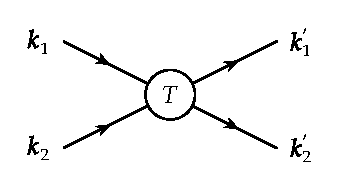
\includegraphics[width=0.45\linewidth]{pictures/4_1}
\par\end{centering}
\caption{\label{fig:T=0077E9=009635=007684=008D39=0066FC=0056FE=008868=00793A}$T$-矩阵的费曼图表示}
 
\end{figure}

可以证明，如果我们考虑两个核子在介质中的散射，定义一个类似于自由粒子散射矩阵的散射矩阵$G^{E}$是有意义的（这是在F.4节中导出的）。对于原子核中的核子，所要做的改变是比较显然的：平面波指标必须改为壳模型指标，方程\ref{eq:Lippmann-Schwinger equation}右侧分母上的单粒子动能必须用相应的壳模型能量来代替，并且中间态的求和范围必须被限制，使得它不包括费米面以下的态。最后一个改动是因为费米面以下的两个核子只能散射到费米面以上的态，因为所有其他能级都被占据
\begin{comment}
由此能量不守恒，所以肯定不行？
\end{comment}
。因此，我们得到下面关于$G$-矩阵的方程，它通常被称为Bethe-Goldstone方程\cite{BG57}（关于它的数学推导，见F.4节）。

\begin{equation}
G^{E}_{ab,cd}=\bar{v}_{ab,cd}+\frac{1}{2}\sum_{m,n>\varepsilon_{\text{F}}}\bar{v}_{ab,mn}\frac{1}{E-\varepsilon_{m}-\varepsilon_{n}+\mathrm{i}\eta}G^{E}_{mn,cd}\label{eq:Bethe-Goldstone equation}
\end{equation}

这里$ab,\dots,mn$是壳模型指标，$\varepsilon_{\text{F}}$是费米能。这个方程用图来表示会比较显然，正如\ref{fig:Bethe-Goldstone=0065B9=007A0B=007684=008D39=0066FC=0056FE=008868=00793A}中那样。连接两个相互作用的两条线代表“传播子''$1/(E-\varepsilon_{n}-\varepsilon_{m})$（在第八章和附录F中会有更详细的关于费曼图的解释）。对于$E<\varepsilon_{\text{F}}$的情况，我们可以忽略\ref{eq:Bethe-Goldstone equation}中分母上的$\mathrm{i}\eta$，在这种情况下$G$-矩阵显然是厄米的，这可以通过迭代利用\ref{eq:Bethe-Goldstone equation}看出。方程\ref{eq:Bethe-Goldstone equation}也可以写成算符形式：

\begin{figure}[H]
\begin{centering}
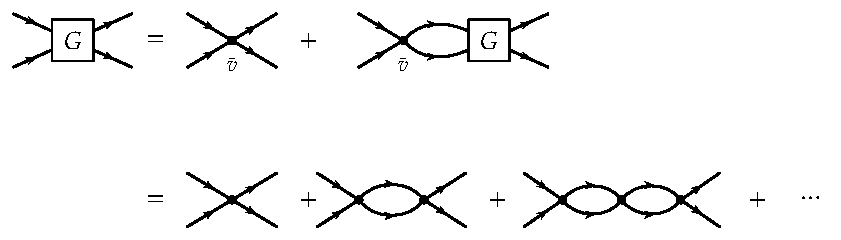
\includegraphics[width=0.7\linewidth]{pictures/4_2}
\par\end{centering}
\caption{\label{fig:Bethe-Goldstone=0065B9=007A0B=007684=008D39=0066FC=0056FE=008868=00793A}Bethe-Goldstone方程的费曼图表示}

\end{figure}

\begin{equation}
G=\bar{v}+\bar{v}\frac{Q_{F}}{E-H_{0}}G\label{eq:operator form Bethe-Goldstone equation}
\end{equation}

这里$H_{0}$是壳模型 Hamilton 量，$Q_{F}$是去掉了所有占据态的投影算符：
\begin{equation}
Q_{F}=\sum_{\begin{subarray}{c}
m<n\\
>\varepsilon_{\text{F}}
\end{subarray}}|mn\rangle\langle mn|\label{eq:project operator}
\end{equation}

我们可以从\ref{eq:operator form Bethe-Goldstone equation}定性地看出当$\bar{v}$无穷大的时候，$G$仍然是有限大的。形式地解\ref{eq:operator form Bethe-Goldstone equation}可以得到：

\[
G=\frac{\bar{v}}{1-\bar{v}Q_{F}/(E-H_{0})}
\]

如果$\bar{v}$是无穷大，$G$仍然是有限大的。这当然是一个粗糙的做法，接下来我们会用一个具体的例子更详细的说明这一点。在此之前，我们必须讨论方程\ref{eq:Bethe-Goldstone equation}的一些性质。尽管\ref{eq:Bethe-Goldstone equation}和\ref{eq:Lippmann-Schwinger equation}形式上很相近，但是还是有一些不同的地方需要注意的，例如类比自由粒子的散射波定义的$E<\varepsilon_{\text{F}}$的的波函数的边界条件{[}Me
61, 第XIX 10章{]}：
\begin{align}
|\psi_{ab}\rangle & \equiv\bar{v}^{-1}G|ab\rangle=\left(1+\frac{Q_{F}}{E-H_{0}}G\right)|ab\rangle\label{eq:G wave function}\\
 & =|ab\rangle+\frac{Q_{F}}{E-H_{0}}\bar{v}|\psi_{ab}\rangle\nonumber 
\end{align}

这里：
\[
\langle\boldsymbol{r}_{1}\boldsymbol{r}_{2}|ab\rangle=\frac{1}{\sqrt{2}}(\varphi_{a}(\boldsymbol{r}_{1})\varphi_{b}(\boldsymbol{r}_{2})-\varphi_{a}(\boldsymbol{r}_{2})\varphi_{b}(\boldsymbol{r}_{1}))
\]

另有：
\[
H_{0}|ab\rangle=(\varepsilon_{a}+\varepsilon_{b})|ab\rangle
\]

方程\ref{eq:G wave function}在形式上类似于散射波的方程。然而，在真正的散射中，式\ref{eq:G wave function}中的第二项给出了波函数的出射部分，因此当两个粒子的相对距离$\left|\boldsymbol{r}_{1}-\boldsymbol{r}_{2}\right|$趋于无穷大时并不为零，但在当前$E<\varepsilon_{F}$的情况下这一项是零。这是因为在真实的散射过程中，方程\ref{eq:Lippmann-Schwinger equation}中的$T$矩阵在得到方程\ref{eq:G wave function}时是“在壳的”，也就是说散射过程前后两个粒子的相对动量的绝对值必须相同，而且$E$必须对应于这个相对动量的值。因此，在真实的散射过程中\ref{eq:G wave function}中的分母可以是零，因此引入了一个奇点。然而这里并不是这样，由于我们假设了$E<\varepsilon_{\text{F}}$，因此方程\ref{eq:G wave function}右边的第二项绝对不可能是“在壳的”，所以它在$\left|\boldsymbol{r}_{1}-\boldsymbol{r}_{2}\right|$很大时变成了零。Day\cite{Da67}的一篇综述里有这些推导，然而，它太长而且也太偏离主题了，不适合在这里讨论。我们因此直接得到：
\[
|\psi^{E}_{ab}\rangle\xrightarrow{\left|\boldsymbol{r}_{1}-\boldsymbol{r}_{2}\right|\rightarrow\infty}|ab\rangle
\]

从方程\ref{eq:G wave function}和\ref{eq:project operator}可以立即得到$a,b<\varepsilon_{\text{F}}$时的归一化条件：
\[
\langle ij|\psi_{ij}\rangle=1\quad i,j<\varepsilon_{F}
\]

把关联对函数$|\psi_{ij}\rangle$用非关联的基展开也是对我们有启发的。从\ref{eq:G wave function}我们可以得到：
\[
|\psi_{ij}\rangle=|ij\rangle+\frac{1}{2}\sum_{mn}C^{ij}_{mn}|mn\rangle
\]

这意味着关联函数不仅包括$|ij\rangle$，也包括费米面以上的成分。可以证明在最重要的应用中$G$矩阵中的$E$都是在费米面以下的。例如，在Brückner-Hartree-Fock理论（第五章）中，我们必须在$i,j<\varepsilon_{\text{F}}$的情况下计算$G^{E=\varepsilon_{i}+\varepsilon_{j}}_{ab,ij}$。我们因此可以在这种情况下用一个简化但精确可解的模型来处理硬核芯，这一模型能展示最重要的特性。

让我们考虑一个非常大的核，它的内部应当和无限大的核也就是核物质非常相似。此外，我们做一个非常粗糙的假设，即相互作用只有一个硬核芯：
\[
\text{当}r\geq c\text{时}V(r)=0\quad\text{且}\quad\text{当}r<c\text{时}V(r)=\infty
\]

此外，我们假设有两个不可分辨粒子，例如一个质子和一个中子，这对于我们要阐释的原理来说以及足够了。现在我们把\ref{eq:G wave function}写成：
\[
(E-H_{0})|\psi_{ab}\rangle=(E-H_{0}+Q_{F}G)|ab\rangle
\]

在我们这种情况（$E=\varepsilon_{i}+\varepsilon_{j}$）下就是：
\begin{equation}
(\varepsilon_{i}+\varepsilon_{j}-H_{0})|\psi_{ij}\rangle=Q_{F}G|ij\rangle=Q_{F}\bar{v}|\psi_{ij}\rangle\label{eq:toy BG equation}
\end{equation}

这里后一个等号我们利用了\ref{eq:G wave function}。上述方程要比一般的Schrödinger方程更难解，因为$Q_{F}$是个非局域的积分算符。这可以在坐标表象下看出：
\[
\langle\boldsymbol{r}_{1}\boldsymbol{r}_{2}|Q_{F}|\boldsymbol{r}^{\prime}_{1}\boldsymbol{r}^{\prime}_{2}\rangle=\sum_{\begin{subarray}{c}
m<n\\
>\varepsilon_{\text{F}}
\end{subarray}}\langle\boldsymbol{r}_{1}\boldsymbol{r}_{2}|mn\rangle\langle mn|\boldsymbol{r}^{\prime}_{1}\boldsymbol{r}^{\prime}_{2}\rangle
\]

在核物质的情况下，方程\ref{eq:toy BG equation}中的单粒子波函数显然是平面波。为了简化，我们也假设单粒子能是纯动能（在介质环境中这并不是一般的情况）。由于平移不变性，核物质质心的移动是平凡的，由此我们得到：
\[
\langle\boldsymbol{r}_{1}\boldsymbol{r}_{2}|\psi_{ij}\rangle\rightarrow\psi_{\boldsymbol{p}_{1}\boldsymbol{p}_{2}}(\boldsymbol{r}_{1}\boldsymbol{r}_{2})=\frac{1}{(2\mathrm{\pi})^{3/2}}\mathrm{e}^{\mathrm{i}\boldsymbol{P}\cdot\boldsymbol{R}}\psi_{\boldsymbol{P}\boldsymbol{p}}(\boldsymbol{r})
\]

这里我们使用了质心系：
\begin{align}
\boldsymbol{P} & =\boldsymbol{p}_{1}+\boldsymbol{p}_{2} & \boldsymbol{p} & =\frac{1}{2}(\boldsymbol{p}_{1}-\boldsymbol{p}_{2})\nonumber \\
\boldsymbol{R} & =\frac{1}{2}(\boldsymbol{r}_{1}+\boldsymbol{r}_{2}) & \boldsymbol{r} & =\boldsymbol{r}_{1}-\boldsymbol{r}_{2}\label{eq:coordinate transformation}
\end{align}

利用所有这些假设，\ref{eq:toy BG equation}变成了：
\begin{align*}
 & \frac{\hbar^{2}}{2m}(p^{2}_{1}+p^{2}_{2}-\nabla^{2}_{1}+\nabla^{2}_{2})\psi_{\boldsymbol{p}_{1}\boldsymbol{p}_{2}}(\boldsymbol{r}_{1}\boldsymbol{r}_{2})\\
= & \frac{1}{(2\mathrm{\pi})^{6}}\int_{p^{\prime}_{1},p^{\prime}_{2}>k_{\text{F}}}\mathrm{d}^{3}\boldsymbol{p}^{\prime}_{1}\mathrm{d}^{3}\boldsymbol{p}^{\prime}_{2}\int\mathrm{d}^{3}\boldsymbol{r}^{\prime}_{1}\mathrm{d}^{3}\boldsymbol{r}^{\prime}_{2}\,\mathrm{e}^{\mathrm{i}(\boldsymbol{p}^{\prime}_{1}\cdot\boldsymbol{r}_{1}+\boldsymbol{p}^{\prime}_{2}\cdot\boldsymbol{r}_{2}-\boldsymbol{p}^{\prime}_{1}\cdot\boldsymbol{r}^{\prime}_{1}-\boldsymbol{p}^{\prime}_{2}\cdot\boldsymbol{r}^{\prime}_{2})}v(\left|\boldsymbol{r}^{\prime}_{1}-\boldsymbol{r}^{\prime}_{2}\right|)\psi_{\boldsymbol{p}_{1}\boldsymbol{p}_{2}}(\boldsymbol{r}^{\prime}_{1}\boldsymbol{r}^{\prime}_{2})
\end{align*}

根据\ref{eq:coordinate transformation}中质心系的变换，我们得到：
\[
\frac{\hbar^{2}}{m}(k^{2}+\nabla^{2}_{\boldsymbol{r}})\mathrm{e}^{\mathrm{i}\boldsymbol{P}\cdot\boldsymbol{R}}\psi_{\boldsymbol{P}\boldsymbol{k}}(\boldsymbol{r})=\frac{1}{(2\mathrm{\pi})^{6}}\int_{\left|\frac{\boldsymbol{P}^{\prime}}{2}\pm\boldsymbol{p}^{\prime}\right|>k_{\text{F}}}\mathrm{d}^{3}\boldsymbol{P}^{\prime}\mathrm{d}^{3}\boldsymbol{p}^{\prime}\mathrm{d}^{3}\boldsymbol{R}^{\prime}\mathrm{d}^{3}\boldsymbol{r}^{\prime}\,\mathrm{e}^{\mathrm{i}[\boldsymbol{P}^{\prime}\cdot(\boldsymbol{R}-\boldsymbol{R}^{\prime})+\boldsymbol{p}^{\prime}\cdot(\boldsymbol{r}-\boldsymbol{r}^{\prime})]}v(r^{\prime})\mathrm{e}^{\mathrm{i}\boldsymbol{P}\cdot\boldsymbol{R}^{\prime}}\psi_{\boldsymbol{P}\boldsymbol{p}}(\boldsymbol{r}^{\prime})
\]

由于$\mathcal{P}^{2}=p^{2}+2pp^{\prime}\cos\theta+p^{\prime2}$，我们看到，即使在限制$p,p^{\prime}>k_{\text{F}}$下，$\mathcal{P}$也可以取从$0$到$\infty$的所有值。对$\boldsymbol{R}^{\prime}$的积分给出$\delta(\boldsymbol{P}-\boldsymbol{\mathcal{P}})$，因此我们也可以执行$\boldsymbol{\mathcal{P}}$积分。由此我们得到以下方程：
\begin{equation}
\frac{\hbar^{2}}{m}\{k^{2}+\Delta_{\boldsymbol{r}}\}\psi_{\boldsymbol{P}\boldsymbol{k}}(\boldsymbol{r})=\frac{1}{(2\mathrm{\pi})^{3}}\int_{\left|\frac{1}{2}\boldsymbol{P}\pm\boldsymbol{p}\right|>k_{\text{F}}}\mathrm{d}^{3}\boldsymbol{p}\,\mathrm{e}^{\mathrm{i}\boldsymbol{p}\cdot\boldsymbol{r}}\int\mathrm{d}^{3}\boldsymbol{r}^{\prime}\,\mathrm{e}^{-\mathrm{i}\boldsymbol{p}\cdot\boldsymbol{r}^{\prime}}v(\boldsymbol{r}^{\prime})\psi_{\boldsymbol{P}\boldsymbol{k}}(\boldsymbol{r}^{\prime})\label{eq:4.56}
\end{equation}

这个方程不仅因为其积分微分结构而比通常的双粒子方程更为复杂，而且还因为波函数对质心动量$\boldsymbol{P}$具有非平凡的依赖性。对于我们的目的而言，将其在$\boldsymbol{P}=0$处求值就足够了。此外，我们可以将\ref{eq:4.56}进行分波展开
\cite[第 X 章第 8 节]{Me61}：
\begin{equation}
\psi_{\boldsymbol{k}}(\boldsymbol{r})=\sum_{lm}\psi_{kl}(r)Y_{lm}(\theta,\varphi)\label{eq:4.57}
\end{equation}

考虑$s$波方程并将\ref{eq:4.56}中的积分拆分为两部分，即$\int^{\infty}_{k_{\text{F}}}=\int^{\infty}_{0}-\int^{k_{\text{F}}}_{0}$，我们得到：
\begin{equation}
\frac{\hbar^{2}}{m}\left(k^{2}+\frac{\partial^{2}}{\partial r^{2}}+\frac{2}{r}\frac{\partial}{\partial r}\right)\psi_{k}(r)=v(r)\psi_{k}(r)-(4\mathrm{\pi})^{2}\int^{k_{\text{F}}}_{0}\frac{\mathrm{d}p\,p^{2}}{(2\mathrm{\pi})^{3}}j_{0}(pr)\int^{\infty}_{0}\mathrm{d}r^{\prime}\,r^{\prime2}j_{0}(pr^{\prime})v(r^{\prime})\psi_{k}(r^{\prime})\label{eq:4.58}
\end{equation}
其中$j_{0}$是最低阶球 Bessel 函数。令$\psi_{k}(r)=(1/r)u_{k}(r)$，我们最终得到：
\begin{equation}
\frac{\hbar^{2}}{m}\left(k^{2}+\frac{\partial^{2}}{\partial r^{2}}\right)u_{k}(r)=v(r)u_{k}(r)-k_{\text{F}}\int^{\infty}_{0}\mathrm{d}r^{\prime}\,\chi(r,r^{\prime})v(r^{\prime})u_{k}(r^{\prime})\label{eq:4.59}
\end{equation}
其中
\begin{equation}
\chi(r,r^{\prime})=\frac{2rr^{\prime}}{\mathrm{\pi}k_{\text{F}}}\int^{k_{\text{F}}}_{0}\mathrm{d}p\,p^{2}j_{0}(pr)j_{0}(pr^{\prime})=\frac{1}{\mathrm{\pi}k_{\text{F}}}\left\{ \frac{\sin k_{\text{F}}(r-r^{\prime})}{r-r^{\prime}}-\frac{\sin k_{\text{F}}(r+r^{\prime})}{r+r^{\prime}}\right\} \label{eq:4.60}
\end{equation}

现在引入以下无量纲量是十分便利的：
\begin{equation}
x=k_{\text{F}}r;\quad x^{\prime}=k_{\text{F}}r^{\prime};\quad K=\frac{k}{k_{\text{F}}};\quad\frac{mv}{k^{2}_{\text{F}}\hbar^{2}}=w\label{eq:4.61}
\end{equation}
这导致
\begin{equation}
\left(\frac{\mathrm{d}^{2}}{\mathrm{d}x^{2}}+K^{2}\right)u_{K}(x)=w(x)u_{K}(x)-\int^{\infty}_{0}\mathrm{d}x^{\prime}\,\chi(x,x^{\prime})w(x^{\prime})u_{K}(x^{\prime})\label{eq:4.62}
\end{equation}

对于有限高度的方势垒，波函数及其一阶导数在势垒边缘处是连续的。我们很容易确信，当势垒高度趋于无穷大时，波函数的一阶导数在边缘处变得不连续，即：
\begin{equation}
u^{\prime}_{K}(c+\epsilon)=A\label{eq:4.63}
\end{equation}
其中$A$是一个常数，$r=c$是硬芯半径，而$\epsilon$是一个无穷小的正量。为了使\ref{eq:4.62}中的$u$产生这种不连续性，乘积$w\cdot u$在$r=c$处必须正比于$\delta$函数。由于对于$r>c$势$w$为零且$u$有限，乘积$w\cdot u$在硬芯半径外部消失。波函数$u$无法穿透到无限硬芯内部（$u\equiv0$）；因为在那里$w=\infty$，乘积$w\cdot u$可以是有限的，记$c^{\prime}=ck_{\text{F}}$，我们可以写出：
\begin{equation}
w(x)u_{K}(x)=A\delta(x-c^{\prime})+l(x)\theta(c^{\prime}-x)\label{eq:4.64}
\end{equation}
函数$l(x)$可以通过要求对于$x<c^{\prime}$，\ref{eq:4.62}的左侧必须为零来确定，因为对于$x<c^{\prime}$有$u\equiv0$。因此由\ref{eq:4.62}结合\ref{eq:4.64}，我们有：
\begin{equation}
l(x)=A\chi(x,c^{\prime})+\int^{c^{\prime}}_{0}\mathrm{d}x^{\prime}\,\chi(x,x^{\prime})l(x^{\prime})\quad(x<c^{\prime})\label{eq:4.65}
\end{equation}
由于硬芯通常相当小（对于$c=0.4\,\text{fm}$在核物质密度下$c^{\prime}=0.57$），我们可以展开\ref{eq:4.65}中的积分核，并从\ref{eq:4.60}得到：
\begin{equation}
\chi(x,x^{\prime})\rightarrow\frac{2xx^{\prime}}{3\mathrm{\pi}}\quad(x<c^{\prime},\;x^{\prime}<c^{\prime})\label{eq:4.66}
\end{equation}
结合\ref{eq:4.66}和\ref{eq:4.65}，我们看到$l(x)$是$c^{\prime2}$量级的，而对$l(x)$的任何积分都将是$c^{\prime3}$量级的。因此在\ref{eq:4.62}中我们可以忽略\ref{eq:4.64}中的第二项，从而得到在$c^{\prime}$的一阶近似下准确的结果：
\begin{align}
\left(\frac{\mathrm{d}^{2}}{\mathrm{d}x^{2}}+K^{2}\right)u_{K}(x) & \simeq A[\delta(x-c^{\prime})-\chi(x,c^{\prime})]+A\chi(x,c^{\prime})\theta(c^{\prime}-x)\nonumber \\
 & =A\frac{2xc^{\prime}}{\mathrm{\pi}}\int^{\infty}_{1}\mathrm{d}p\,p^{2}j_{0}(px)j_{0}(pc^{\prime})+A\chi(x,c^{\prime})\theta(c^{\prime}-x)\nonumber \\
 & =F(x)\label{eq:4.67}
\end{align}
其中我们利用了恒等式：
\begin{equation}
\int^{\infty}_{0}\mathrm{d}p\,p^{2}j_{l}(pr)j_{l}(pr^{\prime})=\frac{\mathrm{\pi}}{2r^{2}}\delta(r-r^{\prime})\label{eq:4.68}
\end{equation}

我们指出，由于\ref{eq:4.67}的右侧仅在$c^{\prime}$的一阶下是精确的，是否保留\ref{eq:4.67}右侧属于二阶项的第二项在某种程度上是任意的。方程\ref{eq:4.67}的通解：
\begin{equation}
u_{K}(x)=\frac{\sin Kx}{K}\int^{x}_{c^{\prime}}\mathrm{d}y\,F(y)\cos Ky-\frac{\cos Kx}{K}\int^{x}_{c^{\prime}}\mathrm{d}y\,F(y)\sin Ky\label{eq:4.69}
\end{equation}
在$x=c^{\prime}$处显然为零。直接代入即可容易地验证方程\ref{eq:4.69}确实是方程\ref{eq:4.67}的解。

解\ref{eq:4.67}与\ref{eq:4.69}中唯一的未知量是常数$A$，我们将通过要求$u_{K}$渐近趋近于未微扰值这一条件\ref{eq:toy BG equation}来确定它。为此，我们首先证明在$x\rightarrow\infty$极限下，\ref{eq:4.69}右侧的第二个积分为零。由于我们在极小$c^{\prime}$的极限下考虑解，我们可以将积分限从$c^{\prime}$到$\infty$取为从$0$到$\infty$，从而有：
\begin{align}
\frac{1}{K}\int^{\infty}_{0}\mathrm{d}y\,F(y)\sin Ky & =\frac{2Ac^{\prime}}{\mathrm{\pi}}\int^{\infty}_{1}\mathrm{d}p\,p^{2}j_{0}(pc^{\prime})\int^{\infty}_{0}\mathrm{d}y\,y^{2}j_{0}(Ky)j_{0}(py)\nonumber \\
 & =\frac{2Ac^{\prime}}{\mathrm{\pi}}\int^{\infty}_{1}\mathrm{d}p\,p^{2}j_{0}(pc^{\prime})\frac{\mathrm{\pi}}{2Kp}\delta(K-p)\nonumber \\
 & =0\label{eq:4.70}
\end{align}
最后的积分之所以消失，是因为$p$在 Fermi 球之外，而$K$在 Fermi 球之内。因此对于$r\rightarrow\infty$，我们发现波函数趋近于未微扰结果（$\psi\rightarrow j_{0}$）当且仅当：
\begin{equation}
\int^{\infty}_{0}\mathrm{d}y\,F(y)\cos Ky=1\label{eq:4.71}
\end{equation}
于是利用\ref{eq:4.67}，我们得到：
\begin{equation}
A=\left\{ \cos Kc^{\prime}-\int^{\infty}_{0}\mathrm{d}y\,\cos(Ky)\chi(y,c^{\prime})\right\} ^{-1}\label{eq:4.72}
\end{equation}
这完成了对硬球势的波函数$u_{K}(x)$的确定。

\begin{figure}[H]
\begin{centering}
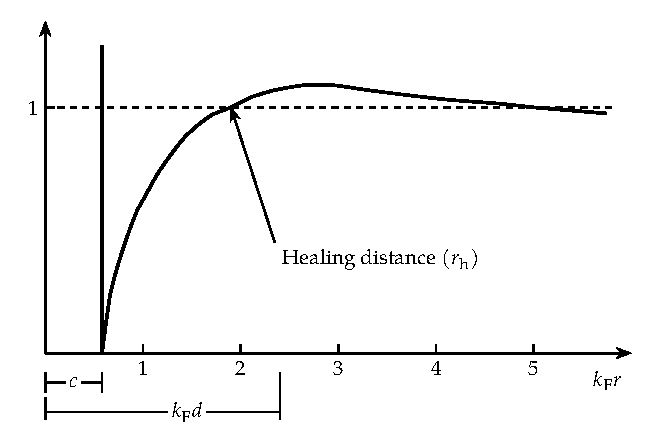
\includegraphics[width=0.65\linewidth]{pictures/4_3}
\par\end{centering}
\caption{\label{fig:4_3}核物质中纯硬芯势的 Bethe–Goldstone 方程的 S 波解。有关图形细节见正文（引自 \cite{FW71}）}
\end{figure}

在图 \ref{fig:4_3} 中，我们展示了对应于$k=0$的解$\psi_{k}(r)$，它揭示了若干有趣的特征。波函数在硬芯内部严格为零。由\ref{eq:4.69}和\ref{eq:4.72}容易看出，它迅速（通过阻尼振荡）趋近于无相互作用核子对的波函数值（对于$k=0$且在所有$r$处该值恒等于
1）。波函数首次达到未微扰值时的$r$值称为\textbf{复原距离}（healing distance）$r_{h}$，因为只有在小于该距离处，硬芯波函数才与未微扰波函数有显著差异。对于我们例子中所选取的数值，复原距离为：
\begin{equation}
k_{\text{F}}r_{h}\simeq1.9\label{eq:4.73}
\end{equation}
（对\ref{eq:4.59}更普遍的研究表明，该值或多或少与$\boldsymbol{P}$和$k$无关 \cite{WG67a}）。值得特别注意的是，这一数值明显小于核物质中的平均粒子间距$d$，后者由表达式$1/d^{3}\equiv N/V=(4\int_{p\le\hbar k_{\text{F}}}\mathrm{d}p\int\mathrm{d}r)/V(2\mathrm{\pi}\hbar)^{3}=2k^{3}_{\text{F}}/(3\mathrm{\pi}^{2})$定义，给出粒子间距为：
\begin{equation}
k_{\text{F}}d=\left(\frac{3\mathrm{\pi}^{2}}{2}\right)^{1/3}=2.46\label{eq:4.74}
\end{equation}

因此平均而言，核子在碰撞之后、下一次碰撞发生之前，就已经恢复为其独立粒子波函数。因此，核波函数的绝大部分由独立粒子波函数构成的行列式组成。这可以视为独立粒子模型合理性的论证——Pauli
原理抑制了散射过程的低动量成分，也就是说，抑制了长程关联。正是由于不相容原理，核子在核内的大多数时间里都表现为独立粒子而运动。Weisskopf
首先指出强相互作用但稀薄的 Fermi 气体中可能发生这种现象 \cite{We50}。

我们已经看到，求解 Bethe–Goldstone 方程\ref{eq:toy BG equation}绝非平凡之事；人们很容易想象，对于波函数不再是平面波且失去平移不变性的有限核，这项任务将变得极其困难。因此目前人们采用了若干近似方案。正如我们在例子中所看到的，正是投影算符$Q_{\text{F}}$使得求解变得十分困难。Moszkowski
与 Scott 的\textbf{分离方法}（separation method）\cite{MS60} 以及 Bethe、Brandow
和 Petschek 的\textbf{参考谱方法}（reference spectrum method）\cite{BBP63}
提出，Pauli 原理应当仅作为微扰来处理。我们不打算深入探讨这些近似方法的细节，读者可参阅 Brown \cite{Br64}、de
Shalit 与 Feshbach \cite{SF74} 的专著以及 Bethe 的综述文章 \cite{Be71}，其中详细阐述了这些方法以及利用谐振子基求解有限核
Bethe–Goldstone 方程等进一步方案。在此我们仅提一下最近在 Brueckner–Hartree–Fock 理论中取得极大成功的另一近似方案（见第
5 章）。这就是 Negele 的\textbf{局域密度近似}（local density approximation, LDA）\cite{Ne70,Ne75}，它最初由
Brueckner、Gammel 和 Weitzner \cite{BGW58} 以及 Brueckner、Lockett 和 Rotenberg
\cite{BLR61} 引入。其基本假设是：有限核中任何局域位置处的$G$矩阵与处于相同密度的无限核物质的$G$矩阵相同，从而在局域上可以像在核物质计算中一样计算$G$矩阵
\cite{Be71,Ne75}。我们将在第 5 章重返这一近似。

\subsection{价核子之间的有效相互作用}

Brueckner $G$矩阵具有重要应用的另一个领域是所谓的\textbf{价核子}之间的有效核力（评述参见 \cite{Ku74b}
及其文献）。作为一个确切的例子，我们考察$^{18}\mathrm{O}$或$^{18}\mathrm{F}$，它们是在双幻核$^{16}\mathrm{O}$芯之上具有两个核子（“价核子”）。在纯壳模型近似中，这两个核子将处于$1d_{5/2}$能级上。我们有望通过使用刚好构成$^{16}\mathrm{O}$芯之上的第一个壳层的$1d_{5/2},2s_{1/2},1d_{3/2}$单粒子态进行组态混合计算，来很好地描述$^{18}\mathrm{O}$的低激发态。此类壳模型计算在第
2 章中已作了一定程度的阐述，并在第 8 章中更详细地处理；例如在第 8 章中我们将证明，这类双价核子体系可以很好地由粒子-粒子 Tamm–Dancoff
久期方程来描述 {[}参见第 8 章式 (8.10){]}：
\begin{equation}
(E^{\text{TD}}_{\rho}-\epsilon_{m}-\epsilon_{n})R^{\rho}_{mn}=\frac{1}{2}\sum_{m^{\prime}n^{\prime}}\bar{v}_{mn,m^{\prime}n^{\prime}}R^{\rho}_{m^{\prime}n^{\prime}}\label{eq:4.75}
\end{equation}
这里的$\epsilon_{m}$是唯象或自洽（见第 5 章）单粒子 Hamilton 量$H_{0}$的单粒子能量，且\ref{eq:4.75}中的所有指标都处于芯的
Fermi 能级以上的\textbf{模型空间}中（在我们的例子中即为$d_{5/2},2s_{1/2},d_{3/2}$态）。对于\ref{eq:4.75}中的双粒子相互作用，我们不能直接采用裸相互作用，因为该力必须模拟并至少近似修正：（a）Fermi
能级以上双粒子组态其余部分的忽略；（b）来自壳模型基更高组态（如$3p-1h,4p-2h$等）的贡献。

下面我们将推导一个精确方程，形式上与\ref{eq:4.75}几乎完全相同，但其中的$\bar{v}$被替换为一个原则上可以从裸相互作用（例如
Hamada–Johnston 势）计算出来的有效（依赖于能量的）相互作用。我们从第 2 章关于壳模型提供一组完全态的结论出发；因此任何精确波函数都可以在该基矢下展开。进行这种展开的一个便捷方法是二次量子化形式，例如$A+2$核子体系态的展开可以写为以下形式（亦见第
8 章；在下文中，指标$m,n,r,p$与$i,j$分别表示处于 Fermi 能级以上和以下的态）：
\begin{align}
|A+2,\tau\rangle & =\sum_{m<n}R^{\tau}_{mn}a^{\dagger}_{m}a^{\dagger}_{n}|\text{HF}\rangle+\sum_{m<n<r,i}R^{\tau}_{mnr,i}a^{\dagger}_{m}a^{\dagger}_{n}a^{\dagger}_{r}a_{i}|\text{HF}\rangle\nonumber \\
 & \quad+\sum_{\begin{subarray}{c}
m<n<r<p\\
i<j
\end{subarray}}R^{\tau}_{mnrp,ij}a^{\dagger}_{m}a^{\dagger}_{n}a^{\dagger}_{r}a^{\dagger}_{p}a_{i}a_{j}|\text{HF}\rangle+\cdots\label{eq:4.76}
\end{align}
此展开中的第一项对应于\ref{eq:4.75}模型空间中保留的态。其它各项则分别代表$3p-1h,4p-2h$等组态。

在第 2 章中我们看到，全部 Slater 行列式的集合同样提供了一组完备态。设精确 Hamilton 量为$H=T+V$，其中$T$为动能，$V$为裸双体相互作用。我们希望对$A+2$粒子体系求解精确
Schrödinger 方程：
\begin{equation}
H|\Psi_{\tau}\rangle=E_{\tau}|\Psi_{\tau}\rangle\label{eq:4.77}
\end{equation}
类似于 Bethe–Goldstone 方程\ref{eq:operator form Bethe-Goldstone equation}，我们将再次利用投影算符来消除未包含在模型空间中的组态。为此我们定义向模型空间（在我们情形中即$2p-0h$态）投影的投影算符$P$：
\begin{equation}
P=\sum_{m<n}a^{\dagger}_{m}a^{\dagger}_{n}|\text{HF}\rangle\langle\text{HF}|a_{n}a_{m}\label{eq:4.78}
\end{equation}
其中指标$m,n$遍历模型空间中包含的所有单粒子态。向 Hilbert 空间的其余部分投影的算符$Q$定义为：
\begin{equation}
Q=1-P\label{eq:4.79}
\end{equation}
利用$P+Q=1$，我们可以将 Schrödinger 方程\ref{eq:4.77}改写为一组耦合方程：
\begin{align}
(E_{\tau}-PHP)P|\Psi_{\tau}\rangle & =PHQ\,Q|\Psi_{\tau}\rangle\label{eq:4.80}\\
(E_{\tau}-QHQ)Q|\Psi_{\tau}\rangle & =QHP\,P|\Psi_{\tau}\rangle\label{eq:4.81}
\end{align}
这就是著名的 Feshbach 投影算符形式 \cite{Fe62}。由于按照假设我们只想计算波函数在模型空间上的投影$P|\Psi_{\tau}\rangle$，我们可以从\ref{eq:4.81}中形式解出$Q|\Psi_{\tau}\rangle$：
\begin{equation}
Q|\Psi_{\tau}\rangle=\frac{1}{E_{\tau}-QHQ}QHP\,P|\Psi_{\tau}\rangle\label{eq:4.82}
\end{equation}
并将此代入\ref{eq:4.80}，从而得到一个完全在模型空间中作用的方程：
\begin{equation}
(PHP+V_{\text{eff}}(E_{\tau}))P|\Psi_{\tau}\rangle=E_{\tau}P|\Psi_{\tau}\rangle\label{eq:4.83}
\end{equation}
其中
\begin{equation}
V_{\text{eff}}(E)=PHQ\frac{1}{E-QHQ}QHP\label{eq:4.84}
\end{equation}

我们看到在方程\ref{eq:4.83}中本征值仍是精确本征值$E_{\tau}$，而波函数只是精确波函数在模型空间上的投影。通过与态$a^{\dagger}_{m}a^{\dagger}_{n}|\text{HF}\rangle$取矩阵元，方程\ref{eq:4.83}可以化为\ref{eq:4.75}的形式。将
Hamilton 量$H$写为$H=H_{0}+V-U$，其中$H_{0}=T+U$为壳模型 Hamilton 量，我们得到：
\begin{equation}
(E_{\tau}-E^{\text{HF}}_{0}-\epsilon_{m}-\epsilon_{n})R^{\tau}_{mn}=\frac{1}{2}\sum_{m^{\prime}n^{\prime}}\langle mn|V_{\text{eff}}(E_{\tau})|m^{\prime}n^{\prime}\rangle R^{\tau}_{m^{\prime}n^{\prime}}\label{eq:4.85}
\end{equation}
其中
\begin{equation}
R^{\tau}_{mn}=\langle\text{HF}|a_{n}a_{m}|\Psi_{\tau}\rangle\label{eq:4.86}
\end{equation}
以及
\begin{equation}
V_{\text{eff}}(E)=P(V-U)P+P(V-U)Q\frac{1}{E-QHQ}Q(V-U)P\label{eq:4.87}
\end{equation}
这里$E^{\text{HF}}_{0}$为芯的 Hartree–Fock 能量，单粒子态选为$H_{0}$的本征态。在推导\ref{eq:4.85}时，我们忽略了$U$的粒子-粒子矩阵元，这在具有较大芯核的情形下是很小的\footnote{$V_{\text{eff}}$的非厄米性质可以通过一种略微不同的定义来避免 {[}参见 Brandow \cite{Br67a}
和 Kuo 等人 \cite{KLR71}{]}。这一引入所谓折叠图（folded diagrams）的形式体系也是不依赖于能量的，但包含了在$G$的高阶项。}。

方程\ref{eq:4.85}具有非线性本征值问题的形式，因为有效相互作用$V_{\text{eff}}$本身依赖于本征值$E_{\tau}$。在实际计算中，通常用平均值$\bar{E}$替代$E_{\tau}$，并将\ref{eq:4.85}作为普通的线性本征值问题求解。投影算符$Q$可以分解为投影到模型空间之外的$2p-0h$态的部分$Q_{2p}$，投影到$3p-1h$态的部分$Q_{3p-1h}$，等等：$Q=Q_{2p}+Q_{3p-1h}+Q_{4p-2h}+\cdots$。如果在\ref{eq:4.87}的投影算符$Q$中只保留$Q_{2p}$并忽略分母中的$U$，则有效相互作用等于将$\epsilon_{\text{F}}$替换为$\epsilon_{\max}$的
Brueckner $G$矩阵\ref{eq:toy BG equation}，即：
\begin{equation}
(V^{(2p)}_{\text{eff}})_{mn,m^{\prime}n^{\prime}}=G^{E^{A+2}_{0}-E^{A}_{0}}_{mn,m^{\prime}n^{\prime}}(\epsilon_{\text{F}}\rightarrow\epsilon_{\max})\label{eq:4.88}
\end{equation}

将精确 Schrödinger 方程改写为\ref{eq:4.85}形式的全部初衷与哲学，均建立在这样一种期望之上：即对于双价核子的物理问题，算符$V_{\text{eff}}$可以通过某种微扰方法在很好近似下计算出来。因此必须假设$V_{\text{eff}}$是良态的，例如它没有强烈的能量依赖性。因此通常忽略\ref{eq:4.88}中$G$的能量依赖，并用下式替代：
\begin{equation}
\Omega_{\tau}\simeq\frac{1}{2}(\epsilon_{m}+\epsilon_{n}+\epsilon_{m^{\prime}}+\epsilon_{n^{\prime}})\label{eq:4.89}
\end{equation}
此外，通常用于求解 Bethe–Goldstone 方程的所有其它近似也不应对结果产生过大影响（参见 \cite{Ma69} 与
\cite{SF74}）。Kuo 与 Brown \cite{KB66} 在谐振子近似下求解了$^{18}\mathrm{O}$和$^{18}\mathrm{F}$的
Bethe–Goldstone 方程，其中裸相互作用采用 Hamada–Johnston 力。随后在\ref{eq:4.85}中利用该力在模型空间中进行对角化，其中单粒子能量取自$^{17}\mathrm{O}$的实验测定值。在图
\ref{fig:4_4} 中，我们给出了这些作者计算的$^{18}\mathrm{O}$低能谱与实验谱的比较；在图 \ref{fig:4_5}
中，我们对$^{210}\mathrm{Pb}$情形展示了同样的结果。后者的计算由 Herling 与 Kuo \cite{HK72}
原则上采用与 Kuo–Brown 相同的方法完成，其模型空间由以下单粒子态构成：

中子：$2g_{9/2},1i_{11/2},1j_{15/2},3d_{5/2},4s_{1/2},2g_{7/2},3d_{3/2}$

质子：$1h_{9/2},2f_{7/2},1i_{13/2},2f_{5/2},3p_{3/2},3p_{1/2}$

\begin{figure}[H]
\begin{centering}
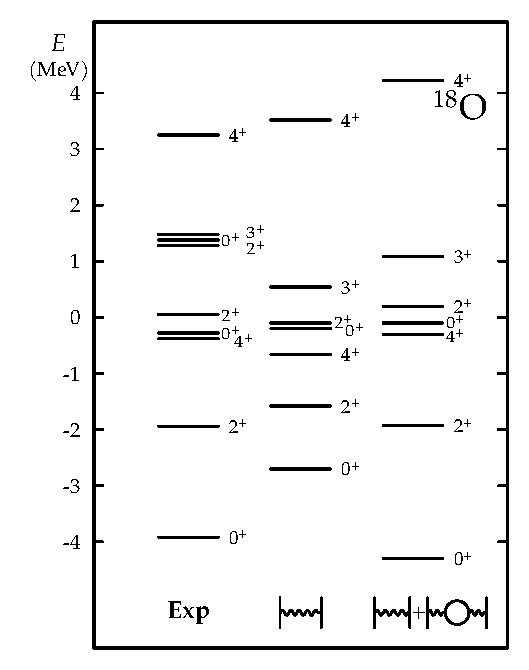
\includegraphics[width=0.5\linewidth]{pictures/4_4}
\par\end{centering}
\caption{\label{fig:4_4}$^{18}\mathrm{O}$的能谱。第一列为实验值；第二列采用纯 $G$ 矩阵计算；第三列同时包含了极化项
(4.90)（引自 \cite{HK72}）}
\end{figure}

\begin{figure}[H]
\begin{centering}
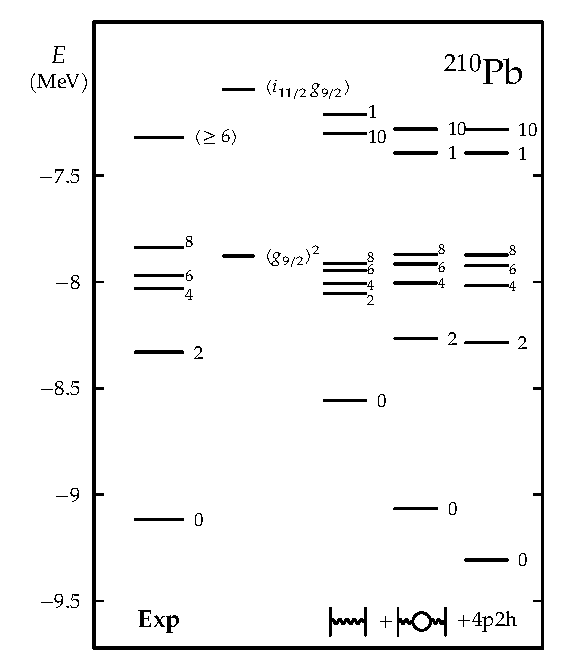
\includegraphics[width=0.55\linewidth]{pictures/4_5}
\par\end{centering}
\caption{\label{fig:4_5}$^{210}\mathrm{Pb}$的能谱。前三列谱的含义与图 \ref{fig:4_4} 相同；在第四列谱中亦考虑了
$4p-2h$ 极化项。图中同时标出了自由双粒子能量（引自 \cite{HK72}）}
\end{figure}

正如从图 \ref{fig:4_4} 和图 \ref{fig:4_5} 中所见，这两项计算与实验的比较并不十分令人满意，其吻合只能被认为是定性的。这种分歧大概并非源于求解
Bethe–Goldstone 方程所引入的各种近似，而是由于忽略了$3p-1h$等其它组态。在上述两项计算中均已表明，至少在微扰论中包含$3p-1h$组态可以极大地改善与实验的一致性。具体步骤是在二阶微扰论中计算\ref{eq:4.83}和\ref{eq:4.85}中来自$Q_{3p-1h}$对$V_{\text{eff}}$的贡献（略去非连通项，见关于折叠图的脚注）。利用我们的定义式，这并不难执行，其结果为：
\begin{equation}
(V^{3p-1h}_{\text{eff}})_{mn,m^{\prime}n^{\prime}}=\left\{ \sum_{pi}\frac{\bar{v}_{mi,m^{\prime}p}\bar{v}_{pn,in^{\prime}}}{\Omega_{\tau}-\epsilon_{m^{\prime}}-\epsilon_{n}-\epsilon_{p}+\epsilon_{i}}-(n^{\prime}\leftrightarrow m^{\prime})\right\} -(m\leftrightarrow n)\label{eq:4.90}
\end{equation}

\begin{figure}[H]
\begin{centering}
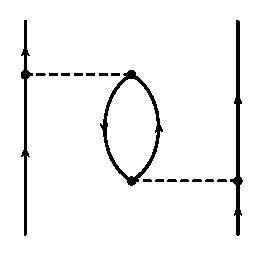
\includegraphics[width=0.28\linewidth]{pictures/4_6}
\par\end{centering}
\caption{\label{fig:4_6}芯极化项的图解表示}
\end{figure}

在这一表达式中，我们忽略了所有使单粒子能量重正化的项，即具有结构$(V_{\text{eff}})_{mn,m^{\prime}n^{\prime}}=A_{mm^{\prime}}B_{nn^{\prime}}-(m^{\prime}\leftrightarrow n^{\prime})$的项，因为通常认为这些项已经包含在具体计算所采用的实验单粒子能中了。通常人们将项\ref{eq:4.90}用图形表示，如图
\ref{fig:4_6} 所示（关于 Feynman 图的更多内容在第 8 章和附录 F 中解释）。然而由于硬芯势的存在，二阶部分不能直接按原样使用。文献
\cite{BK67a} 表明，在$3p-1h$态对$V_{\text{eff}}$的二阶贡献中将裸相互作用替换为其相应的$G$矩阵，正是高阶项的一种自洽重求和。我们在此不详述这些论证，因为它们超出了本书的范围。在图
\ref{fig:4_4} 和图 \ref{fig:4_5} 中也展示了包含这些“重正化”二阶$3p-1h$贡献（即“\textbf{芯极化}”）的结果；可以看出，在两种情形下计算与实验的吻合都近乎完美。如果这就是全部事实，那么结果将是非常令人满意的，因为我们基本上无需引入任何自由参数就解释了这些原子核能谱的低激发部分。

遗憾的是，问题远未彻底解决，因为后续研究表明，包含更高阶项反而会再次使结果恶化。这一效应在图 \ref{fig:4_5} 中清晰体现，其中不仅包含了$3p-1h$项，还包含了$4p-2h$项。Barrett
与 Kirson \cite{BK73} 以及 Kirson 与 Zamick \cite{KZ70} 在这方面进行了更系统但更复杂的深入研究，结果表明不同高阶项的作用导致能谱剧烈涨落，因而无法得出明确结论；特别是，为何二阶$3p-1h$项的引入能与实验达成如此优异的一致性，至今仍未得到彻底阐明。因此人们不得不得出结论：有效相互作用的微观理论仍处于远非令人满意的阶段。

尽管如此，我们仍想回到理论中的两个形式要点。第一点关乎有效相互作用$V^{E}_{\text{eff}}$的能量依赖性。在上述所有计算中，这种能量依赖性或多或少都被忽略了。正如我们已指出的，只要能量依赖性确实很微弱，这种处理当然是成立的。然而实际中$V^{E}_{\text{eff}}$作为$E$的函数可能存在极点，且这些极点可能紧邻甚至落入所关心的低激发态能量区域；例如对于$^{18}\mathrm{O}$即是如此，其中一个集体性的$4p-2h$极点能量降得非常低
\cite{Sch75}。在这种情形下，该极点必须单独处理，因为它在所关心的能量区间内引起了强烈的能量依赖性。这些态在折叠图形式体系中也带来了困难，并被称为\textbf{侵入态}（intruder
states）\cite{SW72,SW73}。在这些情形中，相应有效相互作用按$G$矩阵幂次的微扰展开式极有可能是发散的。人们已经发展了处理这一问题的专门技术
\cite{SW72,SW73,HLR74}。迄今为止我们仅考虑了双核子体系，然而对于多于两个价核子的情形亦可作同样的考量 \cite{Ma69}，尽管我们不打算深入这些细节。

\subsection{粒子-空穴间的有效相互作用}

粒子与空穴间有效相互作用的问题主要出现在闭壳核振动态的研究中（见第 8 章）。然而从微观视角来看，该情形受到的研究远少于价核子之间的相互作用（参见例如
\cite{BK69,KBB70}）。人们可以认为，若能将有效的$ph$力同样用微观$G$矩阵辅以某些高阶修正（如价核子中的极化图）来表示，将是非常理想的。事实上，这一目标确实能够实现。由于在很大程度上，对于$ph$体系被公认为恰当理论的是随机相位近似（RPA，见第
8 章）而非 Tamm–Dancoff 近似（TDA），这使得讨论更为复杂。然而为了不使问题过于繁冗，我们将仅局限于 Tamm–Dancoff
近似情形。

Tamm–Dancoff 方程（见第 8 章）具有以下形式：
\begin{equation}
(E^{\text{TDA}}_{\mu}-\epsilon_{m}+\epsilon_{i})C^{\mu}_{mi}=\sum_{nj}\bar{v}_{mj,in}C^{\mu}_{nj}\label{eq:4.91}
\end{equation}
其中$m,n$（$i,j$）为 Fermi 面以上（以下）的指标。该方程通常在一个模型空间中求解，例如取 Fermi 面之上一壳和之下一壳。类似于双价核子的情形，进入式\ref{eq:4.91}的唯象相互作用必须模拟未包含在模型空间中的$1p-1h$态以及$2p-2h,3p-3h$等态的效应。

一般而言，对于闭壳核我们可以将这种振动态作如下展开（见第 8 章）：
\begin{equation}
|\mu\rangle=\sum_{mi}C^{\mu}_{mi}a^{\dagger}_{m}a_{i}|\text{HF}\rangle+\sum_{\begin{subarray}{c}
m<n\\
i<j
\end{subarray}}C^{\mu}_{mn,ij}a^{\dagger}_{m}a^{\dagger}_{n}a_{i}a_{j}|\text{HF}\rangle+\cdots\label{eq:4.92}
\end{equation}
然而，从式\ref{eq:4.92}出发获得有效相互作用的步骤与价核子情形略有不同。首先我们引入向\textbf{整个}$1p-1h$子空间投影的投影算符$P$：
\begin{align}
P & =\sum_{mi}a^{\dagger}_{m}a_{i}|\text{HF}\rangle\langle\text{HF}|a^{\dagger}_{i}a_{m}\label{eq:4.93}\\
Q & =1-P\nonumber 
\end{align}
其中求和无任何模型空间限制。运用与导出式\ref{eq:4.85}相同的形式体系，我们在$ph$情形下得到：
\begin{equation}
[E_{\mu}-E^{\text{HF}}_{0}-\epsilon_{m}+\epsilon_{i}]C^{\mu}_{mi}=\sum_{nj}\langle mi|V^{E_{\mu}}_{\text{eff}}|nj\rangle C^{\mu}_{nj}\label{eq:4.94}
\end{equation}
其中$V_{\text{eff}}$在形式上由与式\ref{eq:4.83}相同的表达式给出，但投影算符$P$和$Q$改由式\ref{eq:4.93}给出。对$Q$的第一项贡献来自$2p-2h$成分，即来自$Q_{2p-2h}$。计算该项对$V$的二阶微扰贡献，我们得到：
\begin{align}
(V^{(2p-2h)}_{\text{eff}})_{mj,in} & =\sum_{m^{\prime}<n^{\prime}}\bar{v}_{mj,m^{\prime}n^{\prime}}\frac{1}{\Omega_{\mu}+\epsilon_{i}+\epsilon_{j}-\epsilon_{m^{\prime}}-\epsilon_{n^{\prime}}}\bar{v}_{n^{\prime}m^{\prime},in}\nonumber \\
 & \quad-\sum_{i^{\prime}<j^{\prime}}\bar{v}_{j^{\prime}i^{\prime},ni}\frac{1}{\Omega_{\mu}-\epsilon_{m}-\epsilon_{n}+\epsilon_{i^{\prime}}+\epsilon_{j^{\prime}}}\bar{v}_{jm,i^{\prime}j^{\prime}}\nonumber \\
 & \quad-\sum_{n^{\prime}j^{\prime}}\bar{v}_{mj^{\prime},nn^{\prime}}\frac{1}{\Omega_{\mu}-\epsilon_{n}+\epsilon_{i}-\epsilon_{n^{\prime}}+\epsilon_{j^{\prime}}}\bar{v}_{jn^{\prime},ij^{\prime}}\nonumber \\
 & \quad-\sum_{m^{\prime}i^{\prime}}\bar{v}_{ji^{\prime},m^{\prime}i}\frac{1}{\Omega_{\mu}-\epsilon_{m}+\epsilon_{j}-\epsilon_{m^{\prime}}+\epsilon_{i^{\prime}}}\bar{v}_{mm^{\prime},i^{\prime}n}\label{eq:4.95}
\end{align}
其中$\Omega_{\mu}=E^{A}_{\mu}-E^{\text{HF}}_{0}$，且重正化单粒子能的项未包含在内。式\ref{eq:4.95}右端第一项与$V_{\text{eff}}$的一阶项合并，恰好给出$G$矩阵的前两项：
\begin{equation}
G^{\Omega_{\mu}+\epsilon_{i}+\epsilon_{j}}_{mj,in}\label{eq:4.96}
\end{equation}

事实上，我们可以验证，对于$V$的每一阶，在$V_{\text{eff}}$中都存在与式\ref{eq:4.96}相应阶对应的项。因此$V_{\text{eff}}$包含作为第一项的$G$矩阵\ref{eq:4.96}。式\ref{eq:4.95}右端第二项代表空穴-空穴关联，数值计算表明它很小，因而通常可以忽略。第三项和第四项则类似于双价核子情形下的极化图（图
\ref{fig:4_6}）。这些项同样不能直接按原样使用，但我们可以证明，将裸矩阵元替换为其相应的$G$矩阵元是对高阶项的一种自洽重求和。$ph$情形下的极化图如图
\ref{fig:4_7} 所示。在最低阶上我们已经在全$ph$空间中拥有了一个$G$矩阵，这一事实正是$ph$与$pp$情形之间的本质差异。

\begin{figure}[H]
\begin{centering}
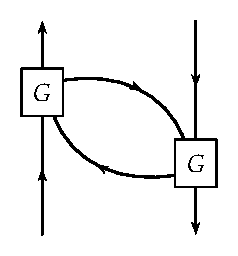
\includegraphics[width=0.28\linewidth]{pictures/4_7}
\par\end{centering}
\caption{\label{fig:4_7}粒子-空穴情形下的极化图}
\end{figure}

认识到这一点后，我们现在可以将方程\ref{eq:4.94}转换为模型$ph$空间中的方程。为此，我们将投影算符$P$拆分为向模型$ph$空间投影的部分$P_{\text{M}}$以及向$ph$空间其余部分投影的部分$P_{\text{R}}$：$P=P_{\text{M}}+P_{\text{R}}$。借助我们已经使用过的
Feshbach 投影算符形式体系 \cite{Fe62} {[}参见式 \ref{eq:4.80} 和 \ref{eq:4.81}{]}，消去方程\ref{eq:4.94}中模型空间之外的成分，即导出一个模型空间中的
TDA 方程。其中出现的有效相互作用可以按$G$矩阵展开到二阶。来自式\ref{eq:4.96}的项示于图 \ref{fig:4_8}，应当注意到对中间态线的求和仅遍历未包含在模型空间中的态。现实的计算
\cite{BK69,KBB70} 表明，包含极化图（图 \ref{fig:4_7}）具有重要效应：不包含它的 RPA 计算（见第
8 章）会给出虚数解，而极化项的贡献使解稳定下来。正如在第 8 章中更详细讨论的，其原因在于 RPA 过高估计了基态关联，必须引入极化项或屏蔽项来降低这些关联。通过这些评述，我们结束对微观有效相互作用的探讨，并在下一节中转向其唯象对应物。

\begin{figure}[H]
\begin{centering}
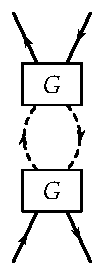
\includegraphics[width=0.28\linewidth]{pictures/4_8}
\par\end{centering}
\caption{\label{fig:4_8}模型 $ph$ 空间中对 $V_{\text{eff}}$ 的二阶贡献。虚线中间态线表示求和仅遍历未包含在模型空间中的态}
\end{figure}


\section{唯象有效相互作用}

\subsection{一般评述}

在第 4.3 节中，我们看到了如何从微观上定义有效核力，以及在实际中计算它们并获得与实验定量吻合的结果是多么困难。因此从核物理发展的早期起，人们就采用了唯象核力，其中包含若干通过拟合实验数据确定的拟合参数（fit
parameters）。在许多情形下，这种做法被证明是极其成功的，仅使用一次性选定并对所有体系通用的少数几个参数，就能解释涵盖甚广的核质量范围内的丰富实验数据。因此，至今仍然缺乏能够令人满意地解释这些唯象核力成功的微观理论，就更显得令人遗憾。

当然，在核物理问题中应用过的唯象相互作用数量极其庞大，每一种相互作用都针对特定问题而使用，其有效性和成功程度大相径庭。给出一个全景图超出了本书的范围，我们将把讨论限制在某些基本性质上，并仅介绍最成功的典型范例。大多数唯象力是专为特定目的构造的，例如用于
Hartree–Fock 计算（见第 5 章），用于计算核自洽场以及核的整体性质（如结合能和饱和密度）；其它相互作用则作为价核子之间或粒子与空穴之间的有效核力（见第
4.3 节）。因此，即使这些不同类型的相互作用在数学结构上看起来非常相似，我们在比较它们时也必须格外审慎。

正如我们在上一节所讨论的，有效相互作用是在特定的壳模型组态空间（即\textbf{模型空间}）中使用的。因此我们必然预期有效相互作用对该空间具有某种依赖性，也就是说，对于不同尺度的模型空间必须选取不同的相互作用。正如我们所见，微观定义的有效相互作用始终是依赖于能量的，而在唯象核力中大部分时间没有显式的能量依赖性，通常将所有这些依赖性归结为一个可变的强度参数就足够了。

显而易见，我们更倾向于将有效相互作用的解析形式选得尽可能简单。例如，人们常常假设有效相互作用遵循与裸核子-核子相互作用相同的\textbf{不变性原理}（见第
4.2 节）。这当然并不总是正确的。例如，我们应当预期描述从裸核子-核子相互作用过渡到有效相互作用的重正化过程依赖于体系的实际密度，也就是说，在体系内部与在表面及外部区域得到的力是不同的。对于在固定势阱中的壳模型计算，我们不应期望剩余相互作用具有平移不变性。

我们知道\textbf{核力的力程}相当短。在第 4.3 节中我们看到，对于有效 $G$ 矩阵的力程而言亦是如此。因此最简单的设想是采用\textbf{零程力}（zero-range
force），其径向依赖由 $\delta$ 函数描述。事实上，这类核力非常有用，因为它们处理极其简便，且能很好地描述许多原子核性质。然而更现实的核力需要具有有限非零的力程
\cite{AS71,Sch72b}。有限力程可以通过\textbf{动量依赖性}来模拟。为了说明这一点，我们将相对距离 $\boldsymbol{r}=\boldsymbol{r}_{1}-\boldsymbol{r}_{2}$
的函数 $V(\boldsymbol{r})$ 变换到动量空间：
\begin{equation}
\langle\boldsymbol{p}|V|\boldsymbol{p}^{\prime}\rangle=\frac{1}{(2\mathrm{\pi}\hbar)^{3}}\int\mathrm{e}^{-\frac{\mathrm{i}}{\hbar}(\boldsymbol{p}-\boldsymbol{p}^{\prime})\cdot\boldsymbol{r}}V(\boldsymbol{r})\,\mathrm{d}^{3}\boldsymbol{r}\label{eq:4.97}
\end{equation}
我们看到 $\delta$ 力在动量空间中是一个常数，而任何力程在动量空间中都表现为 $\boldsymbol{p}$ 依赖性。最简单的转动不变形式为：
\begin{equation}
(2\mathrm{\pi}\hbar)^{3}\langle\boldsymbol{p}|V|\boldsymbol{p}^{\prime}\rangle=V_{0}+V_{1}\boldsymbol{p}^{\prime2}+V_{1}\boldsymbol{p}^{2}+V_{2}\boldsymbol{p}\cdot\boldsymbol{p}^{\prime}\label{eq:4.98}
\end{equation}
在坐标空间中，这对应于动量依赖算符：
\begin{equation}
V(\boldsymbol{r})=V_{0}\delta(\boldsymbol{r})+V_{1}(\hat{\boldsymbol{p}}^{2}\delta(\boldsymbol{r})+\delta(\boldsymbol{r})\hat{\boldsymbol{p}}^{2})+V_{2}\hat{\boldsymbol{p}}\cdot\delta(\boldsymbol{r})\hat{\boldsymbol{p}}\label{eq:4.99}
\end{equation}

有效核力通常依赖于密度 $\rho(\boldsymbol{r})$。例如，如果我们考虑 $G$ 矩阵的表达式 (4.39)，这种\textbf{密度依赖性}便很容易理解：求和的能量范围取决于
Fermi 能，而 Fermi 能本身就是密度的函数。同样容易看出，进入有效相互作用定义的投影算符 $Q$ {[}见式 (4.40)
与 (4.77){]} 可以表示为非局域密度，这是密度依赖性的另一个来源。另一类效果出奇良好的简单形式是\textbf{可分离双体相互作用}，即可以表示为乘积形式（或乘积之和）的核力，其中每个因子仅作用于两个粒子中的一个。

\subsection{简单中心力}

存在大量仅使用中心部分 (4.20) 但径向依赖 $V(r)$ 不同的相互作用。常用的简单势包括例如 Yukawa 势 (4.33)
或：
\begin{align}
V(r) & =-V_{0}\mathrm{e}^{-r^{2}/r^{2}_{0}} & \text{（Gauss 势）}\label{eq:4.100}\\
V(r) & =-V_{0}\frac{\mathrm{e}^{-r/r_{0}}}{1-\mathrm{e}^{-r/r_{0}}} & \text{（Hulthén 势）}\label{eq:4.101}\\
V(r) & =-V_{0}\delta\left(\frac{\boldsymbol{r}}{r_{0}}\right) & \text{（接触势）}\label{eq:4.102}
\end{align}
调节势阱深度 $V_{0}$ 与力程 $r_{0}$ 以拟合实验数据。通常取 $V_{0}\simeq50\,\text{MeV}$
以及 $r_{0}\simeq1\sim2\,\text{fm}$（$\pi$ 介子的 Compton 波长为 $1.4\,\text{fm}$）。

对于式 (4.20) 中依赖于 $r$ 的系数 $V(r)$，通常假定它们具有相同的径向依赖，仅调节其强度与符号以拟合经验数据。在此我们不打算讨论这些混合方案中哪一种是最优的，而仅在表
\ref{tab:=004EA4=006362=006DF7=005408=007CFB=006570} 中给出文献中常用的若干交换混合系数。

\begin{table}[H]
\begin{centering}
\caption{\label{tab:=004EA4=006362=006DF7=005408=007CFB=006570}交换混合系数}
\par\end{centering}
\centering{}%
\begin{tabular}{lcccc}
\hline 
混合类型 & $a_{et}$ & $a_{es}$ & $a_{ot}$ & $a_{os}$\tabularnewline
\hline 
Wigner & 1 & 1 & 1 & 1\tabularnewline
Kurath \cite{Ku56,SW66} & 1 & 0.6 & -0.6 & -1\tabularnewline
Serber \cite{HS57} & 1 & 1 & 0 & 0\tabularnewline
Rosenfeld \cite{EF57} & 1 & 0.6 & -0.34 & -1.78\tabularnewline
Ferrel–Visscher \cite{VF57} & 1 & 0.634 & -0.366 & 0\tabularnewline
Soper \cite{So57} & 1 & 0.46 & 0.14 & -0.4\tabularnewline
Gillet \cite{GGS66} I & 1 & 0.6 & -0.6 & 0.6\tabularnewline
\cite{GGS66} \}II & 1 & 0.4 & -0.2 & 0.2\tabularnewline
\hline 
\end{tabular}
\end{table}


\subsection{Skyrme 相互作用}

这种类型的力最初由 Skyrme \cite{Sk56,Sk59} 提出，用于 Hartree–Fock 计算。为了获得核物质的饱和性质，Skyrme
考虑了一个包含两体力和三体力的有效 Hamilton 量：
\begin{equation}
V=\sum_{i<j}v(i,j)+\sum_{i<j<k}v(i,j,k)\label{eq:4.103}
\end{equation}
三体项取为纯零程形式：
\begin{equation}
v(1,2,3)=t_{3}\delta(\boldsymbol{r}_{1}-\boldsymbol{r}_{2})\delta(\boldsymbol{r}_{2}-\boldsymbol{r}_{3})\label{eq:4.104}
\end{equation}
而两体项是动量空间中的短程展开，其形式类似于式 (4.99)：
\begin{align}
v(1,2) & =t_{0}(1+x_{0}P^{\sigma})\delta(\boldsymbol{r}_{1}-\boldsymbol{r}_{2})+\frac{1}{2}t_{1}[\delta(\boldsymbol{r}_{1}-\boldsymbol{r}_{2})\boldsymbol{k}^{2}+\boldsymbol{k}^{\prime2}\delta(\boldsymbol{r}_{1}-\boldsymbol{r}_{2})]\nonumber \\
 & \quad+t_{2}\boldsymbol{k}^{\prime}\cdot\delta(\boldsymbol{r}_{1}-\boldsymbol{r}_{2})\boldsymbol{k}+\mathrm{i}W_{0}(\boldsymbol{\sigma}_{1}+\boldsymbol{\sigma}_{2})\cdot[\boldsymbol{k}^{\prime}\times\delta(\boldsymbol{r}_{1}-\boldsymbol{r}_{2})\boldsymbol{k}]\label{eq:4.105}
\end{align}
其中动量算符定义为：
\begin{equation}
\boldsymbol{k}=\frac{1}{2\mathrm{i}}(\boldsymbol{\nabla}_{1}-\boldsymbol{\nabla}_{2})\label{eq:4.106}
\end{equation}
它向右侧作用；而
\begin{equation}
\boldsymbol{k}^{\prime}=-\frac{1}{2\mathrm{i}}(\boldsymbol{\nabla}^{\prime}_{1}-\boldsymbol{\nabla}^{\prime}_{2})\label{eq:4.107}
\end{equation}
向左侧作用。相互作用中的六个参数 $t_{0},t_{1},t_{2},t_{3},x_{0},W_{0}$ 必须针对核物质与有限核性质拟合。最后带有
$W_{0}$ 的项表示一个两体自旋-轨道相互作用，正如在第 5 章中将看到的，它在平均场中产生了通常的壳模型单粒子自旋-轨道势。对于自旋饱和的偶偶核，三体项
(4.104) 证明等价于一个密度依赖的双体相互作用\footnote{对于无自旋饱和的体系，这一等价性不再成立。在此类情形下，Skyrme 力中的三体项 (4.107) 是纯局域且排斥的，倾向于自旋平行排列，即核铁磁性。这与观测到的核自旋饱和与配对性质相矛盾。这一困难可以通过采用形如
(4.109) 的密度依赖双体相互作用 \cite{BJS75} 或在三体项中引入非局域性 \cite{ON78} 来避免。}：
\begin{equation}
V_{\rho}(1,2)=\frac{1}{6}t_{3}(1+P^{\sigma})\delta(\boldsymbol{r}_{1}-\boldsymbol{r}_{2})\rho\left(\frac{1}{2}(\boldsymbol{r}_{1}+\boldsymbol{r}_{2})\right)\label{eq:4.109}
\end{equation}

这种密度依赖项也可以看作微观有效相互作用中 $\rho$ 依赖性的唯象表现。这种解释优于认为 Skyrme 力包含三体相互作用的观点，因为我们知道核内的三体相互作用是相当微弱的。过去十多年中，这种力之所以获得如此巨大的重要性，基本上有三个原因：

(i) Vautherin 与 Brink \cite{VB72}（见第 5 章）能够用一套合理的参数复现全元素周期表范围内的结合能，并同时给出正确的核半径。这对于通常不依赖于密度的核力来说此前是无法做到的。

(ii) Negele 与 Vautherin \cite{NV72} 给出了这种核力与前几节所讨论的更基本的 $G$ 矩阵之间的微观联系。

(iii) 该核力的数学形式极其简捷，$\delta$ 函数使各类计算得到了极大的简化。

存在最初由 Moszkowski \cite{Mo70} 提出的类似相互作用，即所谓的\textbf{修正 $\delta$ 相互作用}（modified
$\delta$-interactions, MDI）。它们与 Skyrme 相互作用的区别在于省去了 $t_{2}$ 项和自旋-轨道耦合力，并且具有不同的密度依赖形式（$\sim\rho^{\sigma}$，其中
$\sigma<1$）\footnote{核物质不可压缩性与密度依赖指数 $\sigma$ 之间存在强烈的关联 \cite{CS72}。}。

\subsection{Gogny 相互作用}

尽管 Skyrme 相互作用取得了巨大成功，但人们指出，零程力可能无法模拟现实有效相互作用的长程甚至中程部分。特别是，目前版本的 Skyrme
力无法恰当描述核内的对关联（见第 6 章），因此 Gogny \cite{Go75b} 将 Skyrme 力中的 $t_{0},t_{1},t_{2}$
部分替换为两个带有自旋-同位旋交换混合的 Gauss 函数之和\footnote{Brink 与 Booker \cite{BB67} 最初使用了这一形式；类似密度依赖的有效相互作用在 \cite{Kr70,ZR71,RPS72,LMV73,RBP77}
中亦被广泛采用。}，得到：
\begin{align}
V(1,2) & =\sum^{2}_{i=1}\mathrm{e}^{-(\boldsymbol{r}_{1}-\boldsymbol{r}_{2})^{2}/\mu^{2}_{i}}(W_{i}+B_{i}P^{\sigma}-H_{i}P^{\tau}-M_{i}P^{\sigma}P^{\tau})\nonumber \\
 & \quad+\mathrm{i}W_{0}(\boldsymbol{\sigma}_{1}+\boldsymbol{\sigma}_{2})\cdot[\boldsymbol{k}^{\prime}\times\delta(\boldsymbol{r}_{1}-\boldsymbol{r}_{2})\boldsymbol{k}]\nonumber \\
 & \quad+t_{3}(1+P^{\sigma})\delta(\boldsymbol{r}_{1}-\boldsymbol{r}_{2})\rho^{1/3}\left(\frac{1}{2}(\boldsymbol{r}_{1}+\boldsymbol{r}_{2})\right)\label{eq:4.110}
\end{align}
通过拟合有限核性质和核物质性质确定其参数（见表 \ref{tab:Gogny=00529B=0053C2=006570}）。

\begin{table}[H]
\begin{centering}
\caption{\label{tab:Gogny=00529B=0053C2=006570}Gogny 力参数（D1 参数集）}
\par\end{centering}
\centering{}%
\begin{tabular}{ccccccl}
\hline 
$i$ & $\mu_{i}\,[\text{fm}]$ & $W_{i}$ & $B_{i}$ & $H_{i}$ & $M_{i}\,[\text{MeV}]$ & 其他参数\tabularnewline
\hline 
1 & 0.7 & -402.4 & -100.0 & -496.2 & -23.56 & $W_{0}=+115\,[\text{MeV}\cdot\text{fm}^{5}]$\tabularnewline
2 & 1.2 & -21.30 & -11.77 & 37.27 & -68.81 & $t_{3}=1350\,[\text{MeV}\cdot\text{fm}^{4}]$\tabularnewline
\hline 
\end{tabular}
\end{table}


\subsection{Migdal 力}

这种相互作用由 Migdal \cite{Mi67} 在其有限 Fermi 体系理论中提出。基于 Landau 的 Fermi 液体理论中的相互作用准粒子概念
\cite{La59}，Migdal 引入该相互作用来描述原子核中的集体激发\footnote{详尽展开这一理论将超出本书范围；读者可在第 F.7 节找到某些基本理论成分。}。

从偶偶体系的基态出发，准粒子被定义为相邻奇质量数核中的低激发态。偶偶体系的基态不包含准粒子，而激发态由准粒子占据数 $n_{\lambda}$
来表征。这些占据数发生微小改变 $\delta n_{\lambda}$ 会引起体系总能量 $E_{0}$ 的改变：
\begin{equation}
\delta E_{0}=\sum_{\lambda}\epsilon^{0}_{\lambda}\delta n_{\lambda}+\frac{1}{2}\sum_{\lambda\lambda^{\prime}}F_{\lambda\lambda^{\prime}}\delta n_{\lambda}\delta n_{\lambda^{\prime}}
\end{equation}
其中 $\epsilon^{0}_{\lambda}$ 为在没有任何其它准粒子存在时准粒子 $\lambda$ 的能量，$F_{\lambda\lambda^{\prime}}$
是所谓的准粒子相互作用。Migdal 引入了有效粒子-空穴相互作用 $F^{\omega}$ 以及有效粒子-粒子（或空穴-空穴）相互作用
$F^{\xi}$。在具有平移不变性的无限体系中，准粒子由动量 $\boldsymbol{k}$ 表征，Landau 证明了 $ph$
相互作用 $F(\boldsymbol{k},\boldsymbol{k}^{\prime})$ 由总能量 $E_{0}$ 对准粒子密度
$n(\boldsymbol{k})$ 的二阶导数给出：
\begin{equation}
F^{ph}(\boldsymbol{k},\boldsymbol{k}^{\prime})=\frac{\delta^{2}E_{0}}{\delta n(\boldsymbol{k})\delta n(\boldsymbol{k}^{\prime})}\label{eq:4.111}
\end{equation}
在 Fermi 面上这是一个精确关系。

在有限体系中，准粒子密度 $\bar{\rho}_{\lambda\lambda^{\prime}}$ 不再完全由其对角元（占据数
$n_{\lambda}$）决定，而且还包含了关于单粒子波函数 $\varphi_{\lambda}$ 形式的信息。有效相互作用此时依赖于四个指标，人们建议类比于式
(4.111)，从精确基态能量中导出这一物理量 \cite{Br71}：
\begin{equation}
F^{ph}_{psqr}=\frac{\delta E_{0}}{\delta\bar{\rho}_{qp}\delta\bar{\rho}_{rs}}\label{eq:4.112}
\end{equation}
迄今尚未严格证明这是一个精确关系。然而在截然不同的（近似）理论——小振幅极限下的含时 Hartree–Fock 理论（见第 8.5
节）中，可以导出非常类似的形式：从波函数为 Slater 行列式（即 $\rho^{2}=\rho$，见第 5.3.3 节）且总能量可表示为泛函
$E_{0}[\rho]$ 的假设出发，我们将有效 $ph$ 相互作用获得为 $E_{0}[\rho]$ 对 $\rho$
的二阶泛函导数 {[}式 (8.124){]}，正如在式 (4.112) 中一样。

从上述讨论显而易见，例如 Skyrme 力（第 4.4.3 节）不能直接与 Migdal 力相比，尽管它们在形式上非常相似。然而在近似
$\rho^{2}\simeq\rho$ 下，通过将用 Skyrme 相互作用计算出的基态能量对密度进行两次微商，可以在二者之间建立间接的联系。

与 Skyrme 力类似，Migdal 力是动量空间中的展开。然而与适于 Hartree–Fock 计算的势不同，动量平方项 $p^{2}$
并不起主要作用，因为 Migdal 力无论如何无需保证核物质饱和（它们是专为描述不同物理情景构造的）。在大多数计算中，仅考虑动量空间中的常数项就足够了，这在坐标空间中给出一个纯
$\delta$ 力。另一方面，自旋与同位旋交换混合在此非常重要，它们在粒子-粒子力和粒子-空穴力中是不同的：
\begin{equation}
V(1,2)=V_{0}\delta(\boldsymbol{r}_{1}-\boldsymbol{r}_{2})(f+f^{\prime}\boldsymbol{\tau}^{(1)}\cdot\boldsymbol{\tau}^{(2)}+g\boldsymbol{\sigma}^{(1)}\cdot\boldsymbol{\sigma}^{(2)}+g^{\prime}\boldsymbol{\sigma}^{(1)}\cdot\boldsymbol{\sigma}^{(2)}\boldsymbol{\tau}^{(1)}\cdot\boldsymbol{\tau}^{(2)})\label{eq:4.113}
\end{equation}
$V_{0}$ 是必须针对组态空间调节的强度参数（例如在 $^{208}\mathrm{Pb}$ 区域 $V_{0}=380\,\text{MeV}\cdot\text{fm}^{3}$）。Guman
与 Birbrair \cite{GB65} 提出通过常数 $f,f^{\prime}$ 的线性密度依赖来考虑核内部和外部相互作用强度的差异以及核表面的弥散性：
\begin{equation}
f=f^{\text{ex}}+(f^{\text{in}}-f^{\text{ex}})\rho(r)\label{eq:4.114}
\end{equation}
其中 $\rho(r)$ 具有 Fermi 分布的形式：
\begin{equation}
\rho(r)=\frac{1}{1+\exp[(r-R)/a]}\label{eq:4.115}
\end{equation}
附加参数 $R$ 和 $a$ 分别代表原子核的半径与弥散度。与采用密度依赖相互作用的 Hartree–Fock 计算（见第 5
章）不同，密度 (4.114) 不是自洽调节的。因此 Migdal 力破坏了平移不变性。这当然不是缺点，因为重正化过程与底层的单粒子势紧密相连，而单粒子势同样破坏了平移不变性。事实上，恰当选取有效剩余相互作用应当恢复这一不变性（见
Mikeska 与 Brenig \cite{MB69}）。由这一条件可以推导出参数 $f,f^{\prime},g,g^{\prime}$
之间的额外约束关系 \cite{NW72,NW74}。

Migdal 力已在随机相位近似框架下广泛用于计算原子核的低激发集体振动（见第 8 章）。这类振动产生的有效电荷（见第 9 章）提供了大量的实验数据，用以调节粒子-空穴与粒子-粒子力中的六个参数
$f^{\text{in}},f^{\text{ex}},f^{\prime\text{in}},f^{\prime\text{ex}}$
以及 $g,g^{\prime}$（有关细节参见 \cite{RBS73,BSK73,BER75}）。对于粒子-空穴力，Ring
与 Speth \cite{RS74a} 确定其数值为：
\begin{align}
f^{\text{in}} & =0.0685; & f^{\prime\text{in}} & =0.3315; & f^{\text{ex}} & =-2.165;\nonumber \\
f^{\prime\text{ex}} & =0.465; & g & =0.575; & g^{\prime} & =0.725\label{eq:4.116}
\end{align}
值得注意的是，这是一种未被反对称化的有效 $ph$ 力 \cite{KMS76}。它在原子核外部表现出强烈的吸引，而在原子核内部则接近于零。

\subsection{表面 δ 相互作用（SDI）}

与 Migdal 相互作用类似，表面 $\delta$ 力（Surface-Delta Interaction, SDI）被视为
Fermi 面附近粒子间的有效剩余相互作用。其主要物理思想是：核子在核内部几乎独立运动。事实上，Migdal 的剩余相互作用在核内部确实相当微弱。大部分碰撞发生在核表面，在那里
Pauli 原理失去其重要性，核子感受到强烈的吸引相互作用 \cite{GM65}。力在表面外部的行为再次变得无关紧要，因为那里的波函数具有指数衰减的尾巴，即发现核子的概率迅速趋于零。因此，将整个相互作用限制在核表面上，并定义所谓的\textbf{表面
$\delta$ 相互作用}，是一种十分有意义的物理近似：
\begin{equation}
V(1,2)=-V_{0}\delta(\boldsymbol{r}_{1}-\boldsymbol{r}_{2})\delta(|\boldsymbol{r}_{1}|-R_{0})\label{eq:4.117}
\end{equation}
$V_{0}$ 仍可按通常方式依赖于自旋和同位旋坐标 (4.20)。该力具有非常简单的几何性质。利用 $\delta$ 函数在
Legendre 多项式中的展开：
\begin{equation}
\delta(\boldsymbol{r}_{1}-\boldsymbol{r}_{2})=\frac{\delta(r_{1}-r_{2})}{r_{1}r_{2}}\sum_{l}\frac{2l+1}{4\mathrm{\pi}}P_{l}(\cos\theta_{12})\label{eq:4.118}
\end{equation}
其中 $\theta_{12}$ 为矢量 $\boldsymbol{r}_{1}$ 与 $\boldsymbol{r}_{2}$
之间的夹角，并应用球谐函数的加法定理 \cite[式 4.6.6]{Ed57}，我们得到：
\begin{equation}
V(1,2)=-V_{0}\sum_{lm}\frac{\delta(r_{1}-R_{0})}{r_{1}}Y^{*}_{lm}(\theta_{1},\varphi_{1})\frac{\delta(r_{2}-R_{0})}{r_{2}}Y_{lm}(\theta_{2},\varphi_{2})\label{eq:4.119}
\end{equation}
这是关于可分离项的无穷求和。在球对称基下，耦合到确定角动量的矩阵元变得极其简单，因为在 (4.119) 的求和中只有一项能够幸存下来。该模型力已在诸多计算中得到广泛应用
\cite{KS63,PAM66,FP67,Fa68,VPK69}。它与 Migdal 力一样被用作价核子间的有效核力。然而，将底层的组态空间扩展到多于两个主壳层以上是没有物理意义的，因为在这种情况下我们将遇到具有相同角动量量子数的能级。由于径向积分被波函数在
$r=R_{0}$ 处的值所近似，具有不同径向节点数的波函数之间没有抵消，从而导致这些能级上的粒子感受到非物理的过强相互作用。

\subsection{可分离力与多极展开}

在上一小节中我们看到，表面 $\delta$ 相互作用由于其在壳模型基中的可分离性而变得极其便于处理。如果在二次量子化中相互作用可写为如下形式（符号
$::$ 表示按式 (C.50) 意义下的正规乘积）：
\begin{equation}
V=\,:Q^{\dagger}\cdot Q:\,,\label{eq:4.120}
\end{equation}
其中
\begin{equation}
Q=\sum_{k_{1}k_{2}}q_{k_{1}k_{2}}a^{\dagger}_{k_{1}}a_{k_{2}}\label{eq:4.121}
\end{equation}
为单粒子算符，则我们称核力在\textbf{粒子-空穴方向上可分离}。当其作用于 Slater 行列式时，它产生 $ph$ 对的叠加。如果核力具有形式：
\begin{equation}
V=P^{\dagger}\cdot P\label{eq:4.122}
\end{equation}
其中
\begin{equation}
P^{\dagger}=\frac{1}{2}\sum_{k_{1}k_{2}}p_{k_{1}k_{2}}a^{\dagger}_{k_{1}}a^{\dagger}_{k_{2}}\label{eq:4.123}
\end{equation}
为对产生算符，则称该力在\textbf{粒子-粒子方向上可分离}。当其作用于 Slater 行列式时，产生 $pp$ 对的叠加。像式
(4.120) 和 (4.122) 这样简单的设想似乎很难真实地代表现实核力，然而业已证明，这类示意力在选取适当强度时的矩阵元，与从带有极化项的微观
$G$ 矩阵计算出的矩阵元量级完全一致（见第 4.3 节与附录 F.5）\cite{BK67b}。

在此我们希望进一步研究可分离性问题，并考察不包含自旋与同位旋依赖性的一般唯象有效核力。该核力仅依赖于核子之间的相对距离，因此我们可以按如下方式展开
\cite{La64}：
\begin{equation}
V(|\boldsymbol{r}_{1}-\boldsymbol{r}_{2}|)=\sum_{l}V_{l}(r_{1},r_{2})\sum_{m}Y^{*}_{lm}(\theta_{1},\varphi_{1})Y_{lm}(\theta_{2},\varphi_{2})\label{eq:4.124}
\end{equation}
其中
\begin{equation}
V_{l}(r_{1},r_{2})=2\mathrm{\pi}\int^{1}_{-1}V(|\boldsymbol{r}_{1}-\boldsymbol{r}_{2}|)P_{l}(\cos\theta_{12})\,\mathrm{d}\cos\theta_{12}\label{eq:4.125}
\end{equation}
对于 $\delta$ 力 $V=-V_{0}\delta(\boldsymbol{r})$，我们发现 $V_{l}$ 与 $l$
无关：
\begin{equation}
V_{l}(r_{1},r_{2})=-V_{0}\frac{\delta(r_{1}-r_{2})}{r_{1}r_{2}}\label{eq:4.126}
\end{equation}
在式 (4.124) 中，我们将一般的力写为了无穷项求和，其中每一项在角坐标上都是可分离的。从 $\delta$ 力的情况可以看出，对于短程力我们不能期望这种展开迅速收敛。事实上，如果我们将注意力局限在空间中
$r_{1}\simeq r_{2}\simeq r$ 的较小区域，便可以估计展开式 (4.124) 中每个成分的有效力程。函数
$P_{l}(\cos\theta_{12})$ 的主要贡献仅集中在 $0\le\theta_{12}\lesssim1/l$
的区域（图 \ref{fig:4_9}），也就是说，若势 $V(r_{12})$ 的力程相比于 $r/l$ 很大，则 $V_{l}$
(4.125) 很小；高 $l$ 分量 $V_{l}$ 的强度越大，核力的力程就越短。在零程力（$\delta$ 力）中，所有
$l$ 分量具有相同的相对权重。

\begin{figure}[H]
\begin{centering}
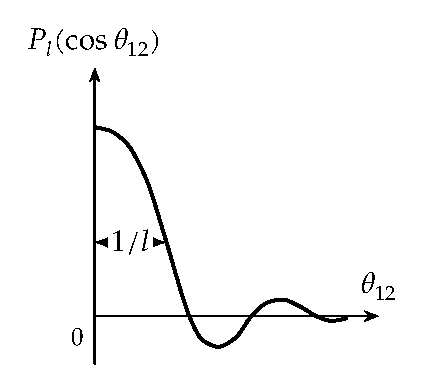
\includegraphics[width=0.42\linewidth]{pictures/4_9}
\par\end{centering}
\caption{\label{fig:4_9}\label{fig:=009636Legendre=00591A=009879=005F0F=005173=004E8E=005939=0089D2=007684=0051FD=006570}$l$
阶 Legendre 多项式作为 $\boldsymbol{r}_{1}$ 和 $\boldsymbol{r}_{2}$ 夹角
$\theta_{12}$ 的函数}
\end{figure}

现在我们回到可分离性问题。由于 $V_{l}(r_{1},r_{2})$ 的径向依赖性，一般的核力 (4.124) 以及 $\delta$
力 (4.126) 并不是可分离的。另一方面，如果假设相互作用具有如 SDI 相互作用 (4.117) 那样在表面尖锐成峰的形式，则由于附加因子
$\delta(r-R_{0})$ 的存在，它便成为可分离项之和：
\begin{equation}
V^{\text{SDI}}_{l}(r_{1},r_{2})=\frac{-V_{0}}{r_{1}}\delta(r_{1}-R_{0})\frac{1}{r_{2}}\delta(r_{2}-R_{0})\label{eq:4.127}
\end{equation}
此类形式的更普遍的可分离设想为：
\begin{equation}
V_{l}(r_{1},r_{2})=f_{l}(r_{1})f_{l}(r_{2})\label{eq:4.128}
\end{equation}
人们通常选取 $f_{l}\sim r^{l}$，并得到\textbf{多极-多极核力}（multipole–multipole
forces）：
\begin{equation}
V=-\frac{1}{2}\sum_{lm}\chi_{l}:Q^{\dagger}_{lm}Q_{lm}:\,=-\frac{1}{2}\sum_{l}\chi_{l}:Q^{\dagger}_{l}\cdot Q_{l}:\label{eq:4.129}
\end{equation}
其中 $\chi_{l}$ 是常数，$Q_{lm}$ 为多极算符：
\begin{equation}
Q_{lm}=\sum_{k_{1}k_{2}}\langle k_{1}|r^{l}Y_{lm}(\theta,\varphi)|k_{2}\rangle a^{\dagger}_{k_{1}}a_{k_{2}}\label{eq:4.130}
\end{equation}
若只考虑具有较小 $l$ 值的成分，我们就获得了\textbf{长程力}。其中最著名的是四极-四极力（quadrupole–quadrupole
force）\cite{El58,KS63}。我们在第 7 章中将看到，它可以用来以自洽的方式描述原子核的四极形变。

我们必须再次强调，这些多极力仅应被视为限制组态空间内价核子之间的有效核力。如果存在许多这样的价核子，我们可以对它们应用 Hartree–Fock
近似\footnote{在此类计算中，HF 势中的交换项 (5.43) 通常因为很小而被忽略 \cite{BK68,Ma74}。}（见第
5 章）。然而，这种针对价核子的多极力 HF 计算绝不能与针对结合能的基础 HF 计算相混淆。

展开式 (4.124) 证明对有效相互作用的\textbf{长程部分}非常有用，因为在此时函数 $V_{l}$ 对较高的 $l$
值变得很小。为了对\textbf{短程部分}获得类似的描述，人们采用另一种不同的展开。我们将把注意力限制在同类核子之间的相互作用（关于质子与中子之间短程关联的处理见第
7.5 节）。我们考察不一定局域的核力的一般表达式 (4.3)：$V(\boldsymbol{r}_{1},\boldsymbol{r}_{2},\boldsymbol{r}^{\prime}_{1},\boldsymbol{r}^{\prime}_{2})$。在局域力的情况下，我们有
$\boldsymbol{r}_{1}=\boldsymbol{r}^{\prime}_{1}$ 以及 $\boldsymbol{r}_{2}=\boldsymbol{r}^{\prime}_{2}$，展开式
(4.124) 是在变量 $\boldsymbol{r}_{1},\boldsymbol{r}_{2}$ 中进行的。现在我们改为要求
$\boldsymbol{r}_{1}=\boldsymbol{r}_{2}$ 以及 $\boldsymbol{r}^{\prime}_{1}=\boldsymbol{r}^{\prime}_{2}$，并在
$\boldsymbol{r}_{1},\boldsymbol{r}^{\prime}_{1}$ 中展开，获得类似于 (4.124)
和 (4.125) 的表达式：
\begin{align}
 & \delta(\boldsymbol{r}_{1}-\boldsymbol{r}_{2})\delta(\boldsymbol{r}^{\prime}_{1}-\boldsymbol{r}^{\prime}_{2})V(\boldsymbol{r}_{1},\boldsymbol{r}^{\prime}_{1})\nonumber \\
= & \,\delta(\boldsymbol{r}_{1}-\boldsymbol{r}_{2})\delta(\boldsymbol{r}^{\prime}_{1}-\boldsymbol{r}^{\prime}_{2})\sum_{lm}V_{l}(r_{1},r^{\prime}_{1})Y_{lm}(\theta_{1},\varphi_{1})Y^{*}_{lm}(\theta^{\prime}_{1},\varphi^{\prime}_{1})\label{eq:4.131}
\end{align}
条件 $\boldsymbol{r}_{1}=\boldsymbol{r}_{2}$ 和 $\boldsymbol{r}^{\prime}_{1}=\boldsymbol{r}^{\prime}_{2}$
已经将我们限制在短程，因为这仅在两个核子处于同一位置时才成立（这并不一定意味着 $\delta$ 力，因为我们允许非局域力）。乍看起来，展开式
(4.131) 对于短程力似乎与式 (4.124) 一样低效。然而，我们必须计算双粒子波函数的矩阵元。正如我们即将证明的，当两个粒子耦合到自旋
$I=l$ 时，(4.131) 中的第 $l$ 项才对矩阵元有贡献。对于单个 $j$ 壳层中的两个粒子而言，例如我们发现当 $I=0$
时它们的波函数具有最大的空间重叠。在此情形下，其波函数的角向部分具有以下形式：
\begin{equation}
\langle\Omega_{1}\Omega_{2}|jjI=0,M=0\rangle\propto\sum^{l}_{m=-l}(-)^{m}Y_{lm}(\Omega_{1})Y_{l,-m}(\Omega_{2})\propto P_{l}(\cos\theta_{12})\label{eq:4.132}
\end{equation}
（由于短程力的性质，我们假设仅自旋单态是重要的）。因此我们发现对于 $I=0$ 相互作用最大，此时角动量 $\boldsymbol{j}_{1}$
与 $\boldsymbol{j}_{2}$ 反平行排列；由此我们可以理解展开式 (4.131) 对于短程相互作用是有重要物理意义的。

同样，如果我们像式 (4.129) 那样将不可分离的径向项替换为可分离设想，即得到：
\begin{equation}
V_{l}(r_{1},r^{\prime}_{1})=-G_{l}r^{l}_{1}r^{\prime l}_{1}\label{eq:4.133}
\end{equation}
由此
\begin{equation}
V=-\sum_{lm}G_{l}P^{\dagger}_{lm}P_{lm}=-\sum_{l}G_{l}P^{\dagger}_{l}\cdot P_{l}\label{eq:4.134}
\end{equation}
其中
\begin{equation}
P^{\dagger}_{lm}=\frac{1}{2}\sum_{k_{1}k_{2}}\langle k_{1}|r^{l}Y_{lm}|\bar{k}_{2}\rangle a^{\dagger}_{k_{1}}a^{\dagger}_{k_{2}}\label{eq:4.135}
\end{equation}
其中 $|\bar{k}\rangle$ 为态 $|k\rangle$ 的时间反演态。在从式 (4.131) 导出式 (4.134)
时，我们必须小心处理自旋坐标 $s$，因为算符 (4.133) 在自旋空间中先验地不是可分离的。然而由于 $\delta$ 力的性质，我们总是有
$s_{1}=-s_{2}$ 以及 $s^{\prime}_{1}=-s^{\prime}_{2}$，这使得推导式 (4.134)
成为可能。

我们现在能够计算单个 $j$ 壳层中 $\delta$ 力的矩阵元，其中单粒子波函数由 $\langle\boldsymbol{r}|nljm\rangle=R_{nl}(r)\langle\Omega|ljm\rangle$
给出。我们构造具有确定角动量 $I,M$ 的对算符 $A^{\dagger}_{IM}$：
\begin{equation}
A^{\dagger}_{IM}=\frac{1}{\sqrt{2}}\sum_{m_{1}m_{2}}C^{j\;\;j\;\;I}_{m_{1}m_{2}M}a^{\dagger}_{jm_{1}}a^{\dagger}_{jm_{2}}\label{eq:4.136}
\end{equation}
并利用式 (4.124) 和 (4.126) 得到：
\begin{equation}
V_{\delta}=-\sum_{I=0,2,\ldots}V_{\delta}(I)\sum_{M}A^{\dagger}_{IM}A_{IM}\label{eq:4.137a}
\end{equation}
其中
\begin{equation}
V_{\delta}(I)=V_{0}\cdot R_{4}\frac{1}{2}\frac{1}{2I+1}|\langle j||Y_{I}||j\rangle|^{2}=\frac{V_{0}}{8\mathrm{\pi}}R_{4}\frac{(2j+1)^{2}}{2I+1}\left|C^{j\;\;\;\;\;j\;\;\;\;\;I}_{1/2\;-1/2\;0}\right|^{2}\label{eq:4.137}
\end{equation}
其中 $R_{4}$ 为径向积分：
\begin{equation}
R_{4}=\int^{\infty}_{0}\mathrm{d}r\,r^{2}R^{4}_{nl}(r)
\end{equation}
从式 (4.137) 可以看出，展开式 (4.131) 中只有第 $l$ 项进入耦合到自旋 $I=l$ 的矩阵元中。在 $\delta$
力的情形下，$V_{\delta}(I)$ 在 $I=0$ 时达到最大值，并随着 $I$ 的增加迅速衰减（表 \ref{tab:Vdelta=0076F8=005BF9=005927=005C0F}）\footnote{在 $I$ 和 $j$ 较大极限下，通过半经典展开可以发现 \cite{MJB75}：$\left|C^{j\;\;\;\;\;j\;\;\;\;\;I}_{1/2\;-1/2\;0}\right|^{2}\simeq\frac{2}{\mathrm{\pi}j}\frac{1}{\sqrt{1-(I/2j)^{2}}}$。}。因此核力
(4.134) 中最重要的部分是 $l=I=0$ 的部分。

\begin{table}[H]
\begin{centering}
\caption{\label{tab:Vdelta=0076F8=005BF9=005927=005C0F}单个 $j$ 壳层中矩阵元 $V_{\delta}(I)$
(4.137) 的相对大小}
\par\end{centering}
\centering{}%
\begin{tabular}{cccccccc}
\hline 
$V_{\delta}(I)/V_{\delta}(0)$ & $I=0$ & 2 & 4 & 6 & 8 & 10 & 12\tabularnewline
\hline 
$j=7/2$ & 1 & 0.238 & 0.117 & 0.058 & — & — & —\tabularnewline
$9/2$ & 1 & 0.242 & 0.126 & 0.075 & 0.040 & — & —\tabularnewline
$11/2$ & 1 & 0.245 & 0.131 & 0.082 & 0.053 & 0.025 & —\tabularnewline
$13/2$ & 1 & 0.246 & 0.133 & 0.087 & 0.060 & 0.038 & 0.019\tabularnewline
\hline 
\end{tabular}
\end{table}

为了避免复杂的公式，人们通常对 Condon–Shortley 相位约定（见 \cite{Ed57}）引入微小修正，即所谓的\textbf{BCS
相位约定}，并对 $m>0$ 定义：
\begin{align}
|nljm\rangle_{\text{BCS}} & =|nljm\rangle_{\text{CS}}\nonumber \\
|nlj-m\rangle_{\text{BCS}} & =(-)^{l+j-m}|nlj-m\rangle_{\text{CS}}\label{eq:BCS phases}
\end{align}
在此约定下，时间反演态 $T|k\rangle$（见式 2.45）对于 $m>0$ 具有极其简单的形式：
\begin{equation}
|\overline{nljm}\rangle=T|nljm\rangle=|nlj-m\rangle;\quad T|nlj-m\rangle=-|nljm\rangle\label{eq:4.139}
\end{equation}
式 (4.134) 的 $l=0$ 部分即为所谓的\textbf{纯配对力}（pure pairing force），它具有以下形式：
\begin{equation}
V^{p}=-G\frac{1}{4}\sum_{\begin{subarray}{c}
kk^{\prime}\\
>0
\end{subarray}}a^{\dagger}_{k^{\prime}}a^{\dagger}_{\bar{k}^{\prime}}a_{\bar{k}}a_{k}\label{eq:pure pairing force}
\end{equation}
其中 $\bar{k}$ 再次为态 $k$ 的时间反演态，求和遍历 $k,k^{\prime}>0$ 的所有取值。该核力在 BCS
形式体系内被广泛用于描述核内的短程关联（见第 6 章）。必须再次指出，它仅适用于受限的组态空间。力常数的值与该空间的大小紧密相关。将这一简单模型力进行推广以包含展开式
(4.131) 中的更高 $l$ 值是容易的，它们被称为\textbf{多极配对力}（multipole pairing forces）。它们在粒子-粒子方向上是可分离的，在配对振动的描述中扮演着重要角色（见第
8 章与 \cite{BB71,BBN74b}）。

通过将四极-四极力与纯配对力相结合，人们获得了用于重核的一个非常简单的模型力——\textbf{配对加四极模型}（pairing-plus-quadrupole
force）\cite{KS60,KS63,BK68}：
\begin{equation}
V^{QP}=-\frac{1}{2}\chi:Q^{\dagger}_{2}\cdot Q_{2}:\,-GP^{\dagger}_{0}\cdot P_{0}\label{eq:4.141}
\end{equation}
它同时考虑了最重要的长程关联与最重要的短程关联，并且处理极其简便（见第 7.4 节）。它基本上包含三个常数：$\chi$ 以及分别针对质子和中子的两个不同配对常数
$G_{p}$ 与 $G_{n}$。它同样只能应用于不大于一个主壳层的组态空间。关于 $\chi$ 和 $G$ 的实际数值参见
\cite{KS60} 或 \cite{BK68}。

\subsection{实验确定的有效相互作用}

由于从裸核子-核子力推导有效相互作用相当繁复，一些作者尝试直接根据实验数据在特定基下确定核子-核子力的矩阵元（综述见 \cite{ST76b}
和 \cite{BPO76}）。

Elliott 等人 \cite{EJM68} 利用核子-核子散射的实验相移，直接在谐振子基下导出了有效相互作用的矩阵元（Sussex
力）。以这种方式，完全避免了硬芯所带来的困难。

较不雄心勃勃但更直接的尝试是根据“简单”原子核的能谱推导特殊的矩阵元。这些核具有充分理由相信其结构仅由少数几个矩阵元决定，这些矩阵元的数目不超过观测到的能级数
\cite{Ta62}。例如我们可以取 $1f_{7/2}$ 壳层核，其中 $f_{7/2}$ 壳层与单粒子谱的其它部分被很好地隔开。人们假设在靠近具有
$N\ge20$ 和 $Z\ge20$ 的双幻芯 $^{40}\mathrm{Ca}$ 的原子核中存在许多纯 $f_{7/2}$
组态。这些能级完全由八个矩阵元 $\langle(f_{7/2})^{2}IT|V|(f_{7/2})^{2}IT\rangle$
决定，其中 $I=0,1,\ldots,7$（对于偶数 $I$ 有 $T=1$；对于奇数 $I$ 有 $T=0$）。McCullen
等人 \cite{MBZ64} 根据 $^{42}\mathrm{Sc}$ 核的能谱确定了这些矩阵元。该核在 $^{40}\mathrm{Ca}$
芯外包含一个中子和一个质子。耦合到总角动量 $I$ 给出相互作用能：
\begin{align}
V(I) & =\langle j_{1}j_{2}I|V|j_{1}j_{2}I\rangle\nonumber \\
 & =B(I,^{42}\mathrm{Sc})-B(I,^{41}\mathrm{Sc})-B(I,^{41}\mathrm{Ca})+B(I,^{40}\mathrm{Ca})\label{eq:4.142}
\end{align}
其中 $B$ 分别为 $^{42}\mathrm{Sc}$ 中自旋为 $I$ 的能级以及其它核基态的实验结合能。利用这些矩阵元，可以相当好地复现具有更多价核子的其它
$f_{7/2}$ 核的许多能级与电磁跃迁性质。然而也遇到了具有更复杂结构（例如 $^{40}\mathrm{Ca}$ 芯中的空穴）的能级，且目前尚不清楚它们在多大程度上与纯
$f_{7/2}$ 组态发生混合。

Schiffer \cite{Sch71b,Sch72b} 以及 Molinari 等人 \cite{MJB75} 对许多这类具有纯组态的简单核进行了更为普遍的研究，其中一个核子处于壳层
$j_{1}$，另一个核子处于壳层 $j_{2}$。角动量的耦合产生自旋满足 $|j_{1}-j_{2}|\le I\le j_{1}+j_{2}$
的多重态。相互作用导致了多重态的能级分裂。为了比较不同的多重态，适宜的做法不是直接绘制 $V(I)$（式 4.137）随 $I$
的变化，而是绘制无量纲比值 $V(I)/\bar{V}$ 作为“重叠角”$\theta_{12}$的函数，其中 $\bar{V}$
是平均双体相互作用能：
\begin{equation}
\bar{V}=\frac{\sum_{I}(2I+1)V(I)}{\sum_{I}(2I+1)}\label{eq:4.143}
\end{equation}
该角度是两价核子经典轨道之间的夹角：
\begin{equation}
\cos\theta_{12}=\frac{\boldsymbol{j}_{1}\cdot\boldsymbol{j}_{2}}{|j_{1}||j_{2}|}=\frac{I(I+1)-j_{1}(j_{1}+1)-j_{2}(j_{2}+1)}{2[j_{1}(j_{1}+1)]^{1/2}[j_{2}(j_{2}+1)]^{1/2}}\label{eq:4.144}
\end{equation}
它度量了两个单粒子波函数的空间重叠。在此类曲线图（图 \ref{fig:4_10}）中，许多不同核的数据点几乎落在同一条曲线上。例如我们给出了两个价核子处于同一轨道时的实验曲线（图
\ref{fig:4_10}a），并将它们与纯 $\delta$ 力的对应理论值（图 \ref{fig:4_10}b）进行比较。对于全同粒子（$T=1$），我们再次发现绝对相互作用矩阵元在
$\theta_{12}=180^{\circ}$ 处最强，即对应于自旋反平行排列（$I=0$），且随着角度减小而迅速下降。对于非全同粒子（$T=0$），相互作用在
$\theta_{12}=0$ 处（即自旋平行排列）同样升高。对于全同粒子，这种构型被 Pauli 原理所禁戒。这体现了短程力要求波函数具有大空间重叠的事实，表明
$\delta$ 型有效相互作用能够定性地再现“实验确定的”矩阵元。然而定量比较 \cite{Sch72b,GSZ74,AEE78}
表明，为了再现奇奇核的性质，还需要引入长程分量。这种长程部分的物理起源目前尚未被完全理解。关于这一观点的深入讨论参见 \cite{Mo76c}。

\begin{figure}[H]
\begin{centering}
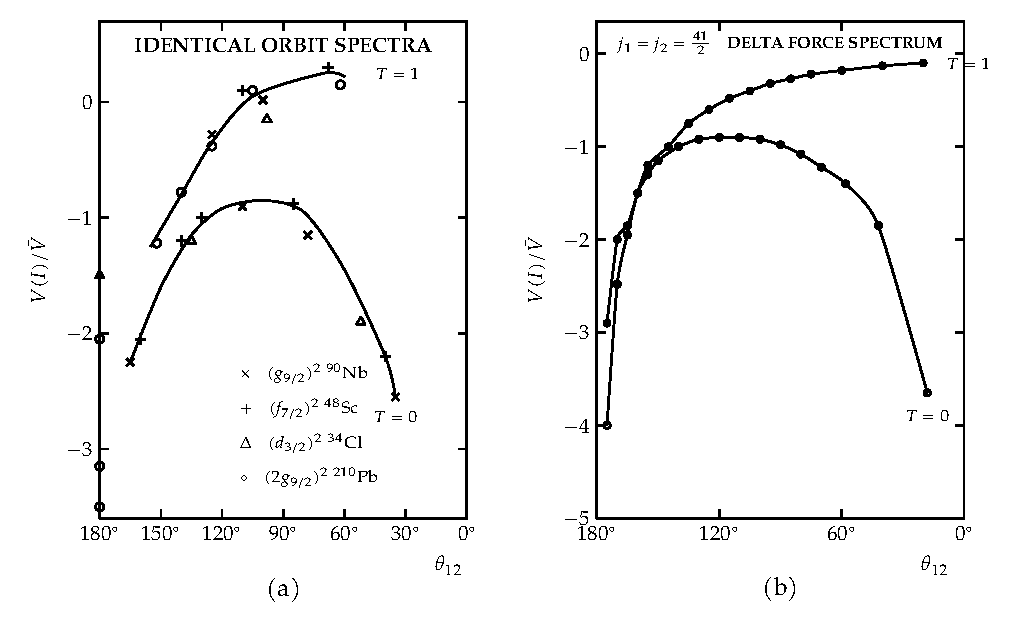
\includegraphics[width=0.78\linewidth]{pictures/4_10}
\par\end{centering}
\caption{\label{fig:4_10}相对相互作用矩阵元 $V(I)/\bar{V}$ 作为重叠角 $\theta_{12}$ 的函数。(a)
四个原子核的实验值；(b) $j_{1}=j_{2}=41/2$ 纯 $\delta$ 力谱（引自 \cite{AS71}）}
\end{figure}


\section{结论}

在本章的第二节中，我们讨论了核子之间的裸相互作用。我们首先限制了它们的解析形式，指出了它们必须服从若干不变性原理。众所周知，核子-核子相互作用的长程部分由单
$\pi$ 介子交换给出；在较短距离下，双 $\pi$ 介子交换以及更重的介子交换开始变得重要。我们没有详述此类研究的最新进展，因为微观裸核子-核子力在核物理中本身构成了一个涉及中能和高能物理的独立学科
\cite{BJ76a}。我们讨论了若干更为传统的唯象设想（通常包含 40 到 50 个拟合参数），它们实现了对核子-核子散射实验数据的完美再现。然而，这种拟合仅向我们提供了关于核力在能壳上（on-shell）行为的信息，而进入多核子体系的离壳（off-shell）部分仍然是不确定的（参见例如
\cite{SS76}）。然而三体计算表明，目前常用的双体相互作用（如 Hamada–Johnston 势或 Reid 软芯势）在离壳行为上彼此差异并不显著。因此我们拥有的唯象裸核子-核子势实际上是相当可靠的。

然而，这些势具有在短距离处强烈排斥的不便特征，因此无法直接应用于核结构计算。多体理论告诉我们应当使用有效力而非裸相互作用，前者实质上是对后者高阶效应的无穷求和。这一步骤不仅以自洽的方式计入了高阶多体效应，而且同时摆脱了硬芯带来的发散困难，因为事实证明有效相互作用是性质优良的。在下一章中我们将看到，有效相互作用概念的应用在计算核基态性质方面取得了相当大的成功，尽管该领域最前沿的纯微观计算（自洽地考虑了三体关联
\cite{KLZ78}）仍未能与实验结合能达成定量的绝对吻合。在所有其它计算中，唯象方法均在某一步骤中被引入。尽管如此，我们可以说该理论对于核基态性质给出了极好的结果。

对于价核子之间有效核力的情形，现状则远没有那么令人满意。例如，在双粒子模型空间内采用唯象双体力进行的壳模型计算能够很好地复现例如 $^{18}\mathrm{O}$
的低激发能谱，我们本可以期望这种成功能够从微观上计算两价核子间有效核力来得到证明。不幸的是，这些尝试仅取得了部分的成功，并表明在相互作用微扰展开的某一阶段与实验达成良好吻合之后，进一步包含更高阶展开项反而会使结果重新恶化。直到目前，在中间阶段达成吻合的原因仍未得到彻底解释。

在这些在数值上极为复杂却仅取得中等成功的微观有效相互作用理论之后，我们在第 4.4 节中转向了唯象有效核力的处理。在那里的情况是相当令人满意的。存在若干唯象设想，它们在解释远多于其拟合参数数量的丰富核实验数据方面取得了极大的成功。其中之一是
Skyrme 力，其在描述核基态性质方面的巨大成功将在下一章中详细讨论。对于核结构计算，我们必须提及非常简捷却高度成功的配对加四极力。在铅同位素区域，准粒子概念似乎工作得非常出色，利用
Migdal 力进行的大量计算所展现的惊人成功充分证明了这一点。像表面 $\delta$ 力这样的简单相互作用，其表现同样出人意料地良好。鉴于它们所取得的巨大成功，从微观视角给出理论解释，显然是一项艰巨却极具挑战性与吸引力的重要任务。
